%==============================================================================
\chapter{Elektrochemische thermodynamica}
\label{ch:elektrochemie}
%==============================================================================

\section{Van chemische naar elektrische energie}

Een spontane reactie verlaagt de Gibbs-energie. In een batterij of brandstofcel verschijnt die daling rechtstreeks als elektrische arbeid, zonder omweg via warmte. Omgekeerd dwingt elektrische arbeid in een elektrolyser een niet-spontane reactie af: waterstof uit water, aluminium uit bauxiet, chloor uit zout. Nieuwe thermodynamica is daarvoor niet nodig. We voegen aan $G$, $\mu$ en $K$ (hoofdstukken~\ref{ch:spontaniteit} en~\ref{ch:reagerend}) alleen de elektrische arbeid toe, en bouwen daarmee cellen, elektrolyse, corrosie en Pourbaix-diagrammen op.

\subsection{Chemische energie als bron van elektrische arbeid}
\label{sec:chemische-elektrische-arbeid}

\subsubsection{Afleiding: waarom $\Delta G$ de maximale niet-expansiearbeid geeft}
\label{sec:afleiding-wmax}

Laat een systeem bij constante $T$ en $p$ naast volumearbeid ook ``extra'' arbeid $\dd{w}_{\text{extra}}$ uitwisselen, bijvoorbeeld elektrische. De eerste hoofdwet en de ongelijkheid van Clausius ($\delta Q \leq T\,\dd{S}$, hoofdstuk~\ref{ch:spontaniteit}) geven
\[
\dd{U} = \delta Q - p\,\dd{V} + \dd{w}_{\text{extra}} \leq T\,\dd{S} - p\,\dd{V} + \dd{w}_{\text{extra}}.
\]
Bij constante $T$ en $p$ is $\dd{U} - T\,\dd{S} + p\,\dd{V} = \dd{G}$, dus $\dd{w}_{\text{extra}} \geq \dd{G}$. De arbeid die het systeem kan \emph{leveren} is hoogstens $-\Delta G$, met gelijkheid in de reversibele limiet:
\begin{equation}
\boxed{\;w_{\max} = -\Delta G\;}
\label{eq:wmax}
\end{equation}

\subsection{Elektrische arbeid en de wet van Faraday}
\label{sec:faraday}

Een lading $Q_e$ die een potentiaalverschil $E$ doorloopt, levert arbeid $Q_e E$. Per mol elektronen is de lading de \emph{constante van Faraday}, $F = N_A e = \SI{96485}{\coulomb\per\mole}$, dus $n$ mol elektronen leveren hoogstens $nFE$.

Omdat elke mol elektronen een vaste hoeveelheid stof omzet, is lading ook stof. Een stroom $I$ gedurende een tijd $t$ zet een massa
\begin{equation}
\boxed{\;m = \frac{I\,t}{nF}\,M\;}
\label{eq:faraday}
\end{equation}
om (\emph{wet van Faraday}, met $n$ elektronen per formule-eenheid). Bij een celspanning $U$ is de elektrische energie per kilogram product
\begin{equation}
\frac{W}{m} = \frac{nFU}{M\,\eta_F},
\label{eq:energie-per-kg}
\end{equation}
met $\eta_F$ het \emph{stroomrendement}: het deel van de lading dat de gewenste reactie dient.

\begin{toepassing}{Waarom aluminium recycleren loont}
Aluminium wordt gemaakt door elektrolyse van $\mathrm{Al_2O_3}$ in gesmolten kryoliet bij \SI{960}{\celsius} (Hall--H\'eroult), met $n = 3$, \SI{4.2}{\volt} en $\eta_F = 0.95$:
\[
\frac{W}{m} = \frac{3 \times 96485 \times 4.2}{0.02698 \times 0.95} = \SI{4.7e7}{\joule\per\kilogram} \approx \SI{13}{\kilo\watt\hour\per\kilogram},
\]
anderhalve dag stroom van een Belgisch gezin voor \'e\'en kilogram metaal. Schroot omsmelten kost minder dan \SI{5}{\percent} daarvan: de Al--O-binding hoeft niet opnieuw verbroken te worden. Koperraffinage daarentegen werkt bij \SI{0.3}{\volt} (koper aan beide elektroden) en kost maar \SI{0.25}{\kilo\watt\hour\per\kilogram}.
\end{toepassing}

\section{De celpotentiaal als thermodynamische grootheid}
\label{sec:celpotentiaal}

In een elektrochemische cel verschijnt $w_{\max} = -\Delta_rG$ volledig als elektrische arbeid $nFE$. Dat geeft de brug tussen chemie en spanning:
\begin{equation}
\boxed{\;\Delta_r G = -n F E\;}
\label{eq:drG-nFE}
\end{equation}
Een positieve celpotentiaal betekent een spontane reactie (galvanische cel); een negatieve vraagt elektrolyse; $E = 0$ is evenwicht.

\begin{figure}[htb]
    \centering
    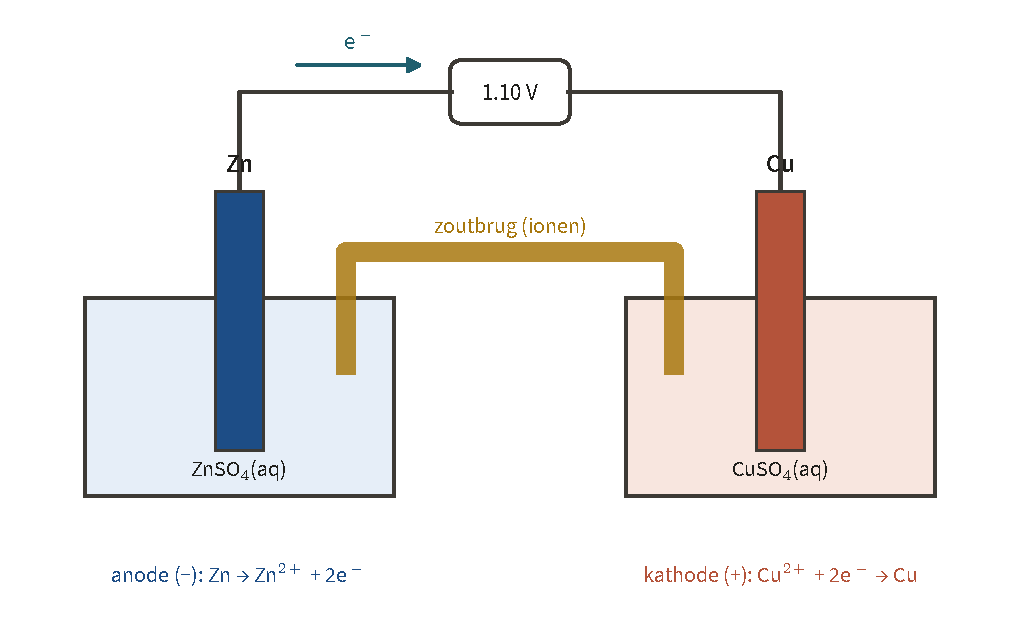
\includegraphics[width=0.8\linewidth]{Figuren/daniell_cel}
    \caption{De Daniell-cel. Zink wordt geoxideerd aan de anode, koperionen worden gereduceerd aan de kathode. Elektronen lopen door de uitwendige draad, ionen door de zoutbrug; samen sluiten ze de stroomkring.}
    \label{fig:daniell-cel}
\end{figure}

\begin{voorbeeld}{De Daniell-cel}
Voor $\mathrm{Zn(s) + Cu^{2+}(aq) \rightarrow Zn^{2+}(aq) + Cu(s)}$ (figuur~\ref{fig:daniell-cel}) is $\Delta_r G^\circ = \SI{-212.3}{\kilo\joule\per\mole}$ en $n = 2$:
\[
E^\circ = -\frac{\Delta_r G^\circ}{nF} = \frac{212\,300}{2 \times 96485} = \SI{1.10}{\volt}.
\]
\end{voorbeeld}

\subsection{De standaardcelpotentiaal en standaardreductiepotentiaal}
\label{sec:standaardreductiepotentiaal}

Een enkele elektrodepotentiaal kan je niet meten, alleen een verschil. Daarom drukt men elke halfreactie uit als \emph{reductiepotentiaal} ten opzichte van de \emph{standaardwaterstofelektrode} (SHE: Pt in $a_{\mathrm{H^+}} = 1$ onder \SI{1}{\bar} \ce{H2}), die per definitie \SI{0}{\volt} is. De celpotentiaal is dan
\begin{equation}
\boxed{\;E^\circ_{\text{cel}} = E^\circ_{\text{kathode}} - E^\circ_{\text{anode}}\;}
\label{eq:Ecel}
\end{equation}
Voor de Daniell-cel: $0.34 - (-0.76) = \SI{1.10}{\volt}$, dezelfde waarde als uit $\Delta_rG^\circ$. Hoe hoger in tabel~\ref{tab:reductiepotentialen}, hoe sterker de oxidator; hoe lager, hoe sterker de reductor.

\begin{table}[htb]
\centering
\small
\begin{tabular}{lc@{\qquad}lc}
\toprule
Halfreactie & $E^\circ$ (V) & Halfreactie & $E^\circ$ (V) \\
\midrule
$\mathrm{F_2 + 2\,e^- \rightarrow 2\,F^-}$ & $+2.87$ & $\mathrm{Cu^{2+} + 2\,e^- \rightarrow Cu}$ & $+0.34$ \\
$\mathrm{Au^+ + e^- \rightarrow Au}$ & $+1.69$ & $\mathrm{2\,H^+ + 2\,e^- \rightarrow H_2}$ & $0.00$ \\
$\mathrm{Cl_2 + 2\,e^- \rightarrow 2\,Cl^-}$ & $+1.36$ & $\mathrm{Fe^{2+} + 2\,e^- \rightarrow Fe}$ & $-0.44$ \\
$\mathrm{O_2 + 4\,H^+ + 4\,e^- \rightarrow 2\,H_2O}$ & $+1.23$ & $\mathrm{Zn^{2+} + 2\,e^- \rightarrow Zn}$ & $-0.76$ \\
$\mathrm{Ag^+ + e^- \rightarrow Ag}$ & $+0.80$ & $\mathrm{Al^{3+} + 3\,e^- \rightarrow Al}$ & $-1.66$ \\
$\mathrm{Fe^{3+} + e^- \rightarrow Fe^{2+}}$ & $+0.77$ & $\mathrm{Na^+ + e^- \rightarrow Na}$ & $-2.71$ \\
 & & $\mathrm{Li^+ + e^- \rightarrow Li}$ & $-3.04$ \\
\bottomrule
\end{tabular}
\caption{Standaardreductiepotentialen bij \SI{298}{\kelvin} (bron: CRC Handbook of Chemistry and Physics).}
\label{tab:reductiepotentialen}
\end{table}

\begin{voorbeeld}{Koper in een zilveroplossing}
Met $E^\circ(\mathrm{Ag^+/Ag}) = \SI{0.80}{\volt}$ als kathode en $E^\circ(\mathrm{Cu^{2+}/Cu}) = \SI{0.34}{\volt}$ als anode is $E^\circ_\text{cel} = \SI{0.46}{\volt}$: $\mathrm{Cu + 2\,Ag^+ \rightarrow Cu^{2+} + 2\,Ag}$ is spontaan. Een koperdraad in zilvernitraat wordt inderdaad met zilverkristallen bedekt.
\end{voorbeeld}

\subsection{De vergelijking van Nernst}
\label{sec:nernst-elektrochemie}

Buiten de standaardtoestand volgt de celpotentiaal uit $\Delta_r G = \Delta_r G^\circ + RT \ln Q$ (hoofdstuk~\ref{ch:reagerend}), gedeeld door $-nF$:
\begin{equation}
\boxed{\;E = E^\circ - \frac{RT}{nF} \ln Q\;}
\label{eq:nernst}
\end{equation}
Bij \SI{298}{\kelvin}, met $\log_{10}$:
\begin{equation}
E = E^\circ - \frac{0.0592}{n} \log_{10} Q.
\label{eq:nernst-log10}
\end{equation}
Een factor tien in $Q$ verschuift de spanning dus met $59/n$ millivolt. Diezelfde \SI{0.0592}{\volt} wordt verderop de helling van de lijnen in een Pourbaix-diagram (\S~\ref{sec:pourbaix-waterlijnen}).

\begin{voorbeeld}{Concentratiecel}
Twee koperelektroden in \SI{0.10}{} en \SI{1.0}{\mole\per\litre} $\mathrm{Cu^{2+}}$: $E^\circ = 0$, maar $E = -\frac{0.0592}{2}\log_{10}(0.10/1.0) = \SI{0.030}{\volt}$. Een concentratieverschil alleen levert al spanning. Zo ontstaat ook corrosie onder een druppel of in een spleet, waar de zuurstofconcentratie lager is.
\end{voorbeeld}

\subsection{De evenwichtsconstante uit de standaardcelpotentiaal}
\label{sec:evenwichtsconstante-elektrochemie}

In evenwicht is $E = 0$ en $Q = K$:
\begin{equation}
\boxed{\;E^\circ = \frac{RT}{nF} \ln K \;\;\Leftrightarrow\;\; \Delta_r G^\circ = -nFE^\circ = -RT \ln K\;}
\label{eq:K-uit-E0}
\end{equation}
Voor $\mathrm{Cu + 2\,Ag^+}$ ($E^\circ = \SI{0.46}{\volt}$, $n = 2$) is $\ln K = 2 \times 96485 \times 0.46/(8.314 \times 298) = 35.8$, dus $K \approx 4\times10^{15}$: de reactie loopt volledig af. Een spanning van enkele tienden volt betekent al een enorme $K$.

\subsubsection{Temperatuursafhankelijkheid van de celpotentiaal: $\Delta_rS^\circ$ en $\Delta_rH^\circ$ zonder calorimetrie}
\label{sec:temperatuur-E}

Leid $\Delta_rG^\circ = -nFE^\circ$ af naar $T$ en gebruik $(\partial \Delta_rG^\circ/\partial T)_p = -\Delta_rS^\circ$:
\begin{gather}
\boxed{\;\Delta_rS^\circ = nF\left(\frac{\partial E^\circ}{\partial T}\right)_p\;}
\label{eq:dSdE}\\
\Delta_rH^\circ = \Delta_rG^\circ + T\Delta_rS^\circ = -nFE^\circ + nFT\left(\frac{\partial E^\circ}{\partial T}\right)_p
\label{eq:dH-uit-E}
\end{gather}
Een spanningsmeting bij enkele temperaturen geeft dus $\Delta_rG^\circ$, $\Delta_rS^\circ$ \'en $\Delta_rH^\circ$, zonder calorimeter. Voor de Daniell-cel is $\partial E^\circ/\partial T \approx \SI{-1.1e-4}{\volt\per\kelvin}$, zodat $\Delta_rS^\circ = 2 \times 96485 \times (-1.1\times10^{-4}) \approx \SI{-21}{\joule\per\mole\per\kelvin}$ en $\Delta_rH^\circ = -212.3 + 298 \times (-0.021) \approx \SI{-218.5}{\kilo\joule\per\mole}$, in overeenstemming met de vormingsenthalpie\"en.

\section{Elektrolyse en de thermodynamische minimumspanning}

Een niet-spontane reactie ($\Delta_r G > 0$) kan je afdwingen met een uitwendige spanning van minstens $\Delta_r G/nF$. In de praktijk is meer nodig, door overspanning aan de elektroden en weerstand in elektrolyt en membraan (\S~\ref{sec:elektrodekinetiek}).

\begin{voorbeeld}{Elektrolyse van water}
Voor $\mathrm{2\,H_2O(l) \rightarrow 2\,H_2(g) + O_2(g)}$ is $\Delta_r G^\circ = \SI{+474.4}{\kilo\joule\per\mole}$ en $n = 4$:
\[
E^\circ_{\text{min}} = \frac{474\,400}{4 \times 96485} = \SI{1.23}{\volt}.
\]
Industri\"ele elektrolysers werken bij \SIrange{1.7}{2.2}{\volt}, vooral door de overspanning aan de zuurstofelektrode.
\end{voorbeeld}

\paragraph{Omkeerbare en thermoneutrale spanning.} De \SI{1.23}{\volt} dekt enkel $\Delta_rG^\circ$. De reactie vraagt in totaal $\Delta_rH^\circ = \SI{571.6}{\kilo\joule}$; het verschil $T\Delta_rS^\circ$ moet als warmte binnenkomen. Levert de stroom ook die warmte, dan is $U_\mathrm{tn} = \Delta_rH^\circ/nF = \SI{1.48}{\volt}$, de \emph{thermoneutrale spanning}. Figuur~\ref{fig:waterstof-spanning} vertaalt elke spanning met Faraday naar elektriciteit per kilogram waterstof.

\begin{figure}[htb]
    \centering
    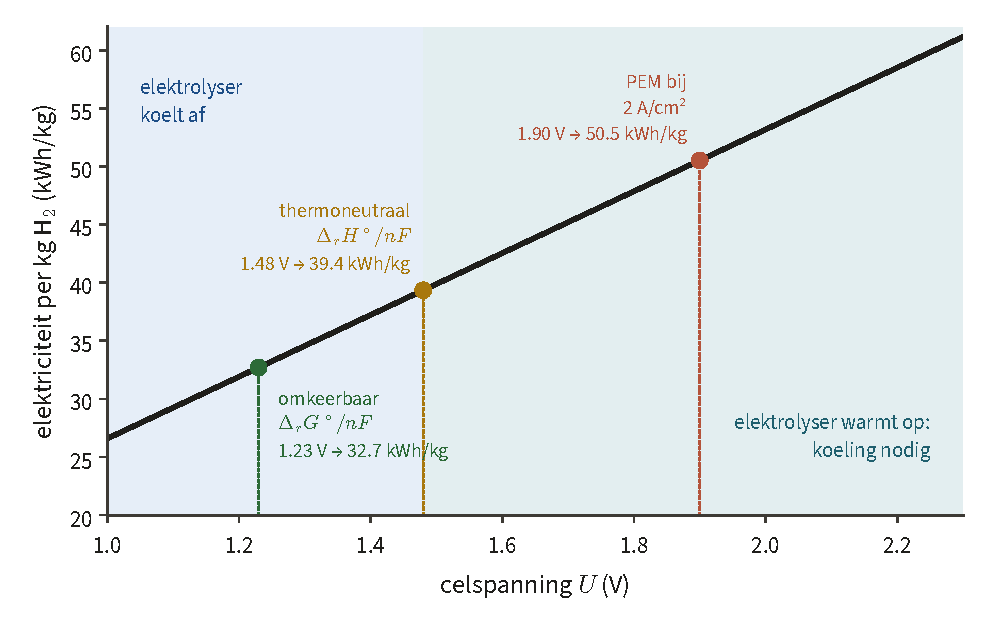
\includegraphics[width=0.72\linewidth]{Figuren/waterstof_spanning}
    \caption{Elektriciteitsverbruik per kilogram waterstof in functie van de celspanning (vergelijking~\eqref{eq:energie-per-kg} met $n = 2$, $\eta_F = 1$). Bij \SI{1.48}{\volt} is het verbruik gelijk aan de verbrandingswarmte (HHV) van waterstof. Daaronder koelt de elektrolyser af, daarboven moet hij gekoeld worden.}
    \label{fig:waterstof-spanning}
\end{figure}

\subsection{De galvanische cel en de batterij}

In een galvanische cel zijn oxidatie (aan de \emph{anode}) en reductie (aan de \emph{kathode}) ruimtelijk gescheiden, zodat de elektronen door een uitwendige kring moeten. Een \emph{batterij} is zo'n cel, gebouwd om energie op te slaan. Primaire batterijen (alkalisch Zn--\ce{MnO2}) ontlaad je \'e\'en keer; secundaire (lood, lithium-ion) laad je op door elektrolyse in de omgekeerde richting.

\begin{voorbeeld}{Hoeveel energie past er in een kilogram batterij?}
De loodaccu werkt met $\mathrm{Pb + PbO_2 + 2\,H_2SO_4 \rightleftharpoons 2\,PbSO_4 + 2\,H_2O}$, $E^\circ = \SI{2.04}{\volt}$ (zes cellen geven \SI{12}{\volt}). Het vaste \ce{PbSO4} blijft op de elektroden zitten, daarom is hij herlaadbaar. Met $n = 2$ en \SI{642.6}{\gram} reagentia:
\[
\frac{2 \times 96485 \times 2.04}{0.6426} = \SI{6.1e5}{\joule\per\kilogram} = \SI{170}{\watt\hour\per\kilogram}.
\]
Voor lithium-ion ($\mathrm{LiC_6 + CoO_2 \rightarrow C_6 + LiCoO_2}$, $n = 1$, \SI{3.7}{\volt}, \SI{169.9}{\gram}) is dat \SI{580}{\watt\hour\per\kilogram}. Echte cellen halen een kwart (lood: \SIrange{30}{40}{\watt\hour\per\kilogram}) tot de helft (Li-ion: \SIrange{150}{270}{\watt\hour\per\kilogram}) van de theorie. Hoge spanning en lichte elementen maakten de elektrische auto mogelijk.
\end{voorbeeld}

\subsection{Brandstofcellen}

Een \emph{brandstofcel} zet continu toegevoerde brandstof (meestal \ce{H2}) en zuurstof om in stroom: de omgekeerde waterelektrolyse, met $E^\circ = \SI{1.23}{\volt}$. Een PEM-cel levert in de praktijk \SIrange{0.6}{0.8}{\volt}, door dezelfde kinetische verliezen.

\section{Elektrodekinetiek in het kort: waarom de spanning afwijkt}
\label{sec:elektrodekinetiek}

Thermodynamica geeft de spanning bij stroom nul. Met stroom verliest een galvanische cel spanning en vraagt een elektrolyser er extra. Dat verschil met de evenwichtspotentiaal heet \emph{overspanning} $\eta$, met drie bronnen:
\begin{itemize}
\item \textbf{activering}: elektronenoverdracht heeft een activeringsenergie (hoofdstuk~\ref{ch:kinetiek});
\item \textbf{ohmse verliezen}: elektrolyt, membraan en contacten hebben weerstand, verlies $iR$;
\item \textbf{concentratie}: bij hoge stroom raken de reagentia aan het oppervlak op; diffusie begrenst de stroom.
\end{itemize}
Voor de activeringsoverspanning geldt bij voldoende stroom de \emph{vergelijking van Tafel}:
\begin{equation}
\boxed{\;\eta = b\,\log_{10}\frac{i}{i_0}\;}
\label{eq:tafel}
\end{equation}
met $i$ de stroomdichtheid, $b$ de \emph{Tafelhelling} (\SIrange{0.03}{0.12}{\volt} per decade) en $i_0$ de \emph{uitwisselingsstroomdichtheid}: hoe snel de reactie in evenwicht heen en terug gaat. Die hangt sterk af van het elektrodemateriaal: voor waterstofontwikkeling \SI{e-3}{\ampere\per\centi\metre\squared} op platina, \SI{e-12}{} op kwik. Een elektrokatalysator verhoogt $i_0$ zonder de evenwichtspotentiaal te veranderen, zoals elke katalysator.

\begin{figure}[htb]
    \centering
    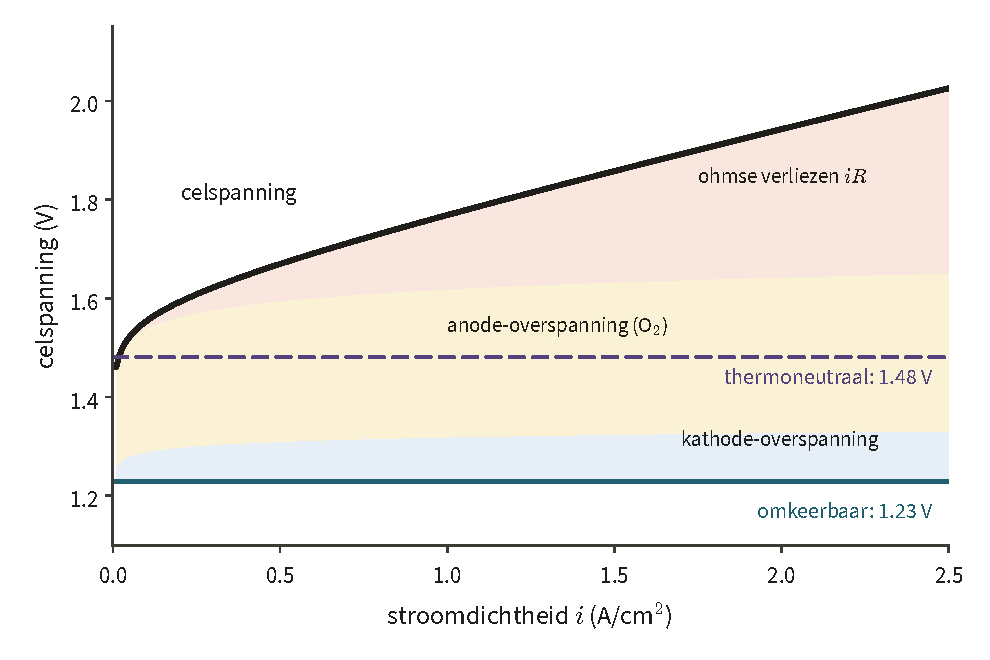
\includegraphics[width=0.75\linewidth]{Figuren/elektrolyser_polarisatie}
    \caption{Celspanning van een PEM-elektrolyser als functie van de stroomdichtheid, opgesplitst in de omkeerbare spanning en de drie verliezen (illustratieve parameters). De zuurstofelektrode is de grootste kinetische rem; bij hoge stroom wegen de ohmse verliezen door.}
    \label{fig:elektrolyser-polarisatie}
\end{figure}

\begin{toepassing}{Rendement van elektrolysers en brandstofcellen}
Een PEM-elektrolyser bij \SI{2}{\ampere\per\centi\metre\squared} werkt rond \SI{1.9}{\volt} (figuur~\ref{fig:elektrolyser-polarisatie}): een rendement van $1.48/1.9 = \SI{78}{\percent}$ (HHV). Een brandstofcel bij \SI{0.7}{\volt} haalt $0.7/1.48 = \SI{47}{\percent}$. De keten stroom $\rightarrow$ waterstof $\rightarrow$ stroom verliest dus meer dan de helft. De ontwerper kiest telkens tussen een grote stroomdichtheid (kleine, goedkope stack) en een lage spanning (hoog rendement).
\end{toepassing}

Corrosie is ook een elektrodeproces, en daar komt dezelfde kinetiek terug (\S~\ref{sec:corrosiesnelheid}).

\section{Corrosie en het Pourbaix-diagram}

\subsection{Corrosie als spontane galvanische cel}
\label{sec:corrosie-galvanisch}
\label{sec:corrosie}

Corrosie is een galvanische cel die niemand wil: het metaal is de anode en wordt geoxideerd, terwijl zuurstof of H$^+$ wordt gereduceerd. Voor ijzer in belucht water:
\begin{align}
\mathrm{Fe} &\rightarrow \mathrm{Fe^{2+}} + 2\,e^-, & E^\circ&=\SI{-0.44}{\volt}\ \text{(reductiepotentiaal, tabel~\ref{tab:reductiepotentialen})},\\
\mathrm{O_2 + 4\,H^+ + 4\,e^-} &\rightarrow \mathrm{2\,H_2O}, & E^\circ&=\SI{1.23}{\volt}.
\end{align}

\begin{voorbeeld}{De drijvende kracht achter roestvorming}
De volledige corrosiereactie is $\mathrm{2\,Fe + O_2 + 4\,H^+ \rightarrow 2\,Fe^{2+} + 2\,H_2O}$, met $n=4$. De standaardcelpotentiaal bedraagt
\[
E^\circ_{\text{cel}} = E^\circ_{\text{kathode}} - E^\circ_{\text{anode}} = \SI{1.23}{\volt} - (\SI{-0.44}{\volt}) = \SI{1.67}{\volt}.
\]
We passen de Nernstvergelijking~\eqref{eq:nernst} toe op typische omstandigheden: neutraal water (pH~7, dus $a_{\mathrm{H^+}}=10^{-7}$), lucht ($p_{\mathrm{O_2}}\approx\SI{0.21}{\bar}$) en een spoor opgelost $\mathrm{Fe^{2+}}$ ($a_{\mathrm{Fe^{2+}}}\approx10^{-6}$):
\[
Q = \frac{a_{\mathrm{Fe^{2+}}}^2}{p_{\mathrm{O_2}}\cdot a_{\mathrm{H^+}}^4} = \frac{(10^{-6})^2}{(0.21)(10^{-7})^4} \approx 4.8\times10^{16}.
\]
\[
E = E^\circ_{\text{cel}} - \frac{RT}{nF}\ln Q = \SI{1.67}{\volt} - \frac{(\SI{8.314}{})( \SI{298}{})}{(4)(\SI{96485}{})}\ln(4.8\times10^{16}) \approx \SI{1.42}{\volt}.
\]
Ook onder realistische omstandigheden blijft $E$ sterk positief ($\Delta_rG \approx \SI{-549}{\kilo\joule\per\mole}$). De thermodynamica biedt geen enkele rem: bescherming (verf, coatings, legeren, kathodische bescherming, \S~\ref{sec:sturen-stabiliteit}) is onmisbaar.
\end{voorbeeld}

\subsection{Hoe snel corrodeert een metaal?}
\label{sec:corrosiesnelheid}

De thermodynamica zegt \emph{of} een metaal corrodeert; de ingenieur wil weten \emph{hoeveel millimeter per jaar}. Omdat corrosie een elektrochemische reactie is, volgt de snelheid rechtstreeks uit de \emph{corrosiestroomdichtheid} $i_\mathrm{corr}$ en de wet van Faraday (vergelijking~\eqref{eq:faraday}). Delen door de dichtheid $\rho$ geeft de dikte die per tijdseenheid verdwijnt:
\begin{equation}
\boxed{\;v_\mathrm{corr} = \frac{i_\mathrm{corr}\,M}{nF\rho}\;}
\label{eq:corrosiesnelheid}
\end{equation}

\begin{voorbeeld}{Van microampère naar millimeter per jaar}
Voor staal ($M = \SI{55.85}{\gram\per\mole}$, $n=2$, $\rho = \SI{7.87}{\gram\per\centi\metre\cubed}$) en $i_\mathrm{corr} = \SI{1}{\micro\ampere\per\centi\metre\squared}$:
\[
v_\mathrm{corr} = \frac{(\SI{e-6}{\ampere\per\centi\metre\squared})(\SI{55.85}{\gram\per\mole})}{(2)(\SI{96485}{\coulomb\per\mole})(\SI{7.87}{\gram\per\centi\metre\cubed})} = \SI{3.7e-11}{\centi\metre\per\second} = \SI{0.012}{\milli\metre}/jaar.
\]
Een handige vuistregel: \SI{1}{\micro\ampere\per\centi\metre\squared} komt voor staal overeen met ongeveer \SI{12}{\micro\metre} per jaar. Onbeschermd staal in zeewater corrodeert met \SIrange{0.1}{0.2}{\milli\metre}/jaar, dus \SIrange{10}{20}{\micro\ampere\per\centi\metre\squared}. Daarom voorziet de ontwerper van een drukvat of leiding een \emph{corrosietoeslag}: typisch \SI{3}{\milli\metre} extra wanddikte voor twintig jaar dienst.
\end{voorbeeld}

Waar komt $i_\mathrm{corr}$ vandaan? Op een corroderend metaal lopen twee reacties tegelijk: de oxidatie van het metaal (anodisch) en de reductie van zuurstof of H$^+$ (kathodisch). Er loopt geen netto stroom naar buiten, dus beide stromen zijn even groot. Het metaal neemt vanzelf de potentiaal aan waar dat zo is: de \emph{corrosiepotentiaal} $E_\mathrm{corr}$. Een \emph{Evansdiagram} (figuur~\ref{fig:evans}) zet beide Tafellijnen uit tegen de logaritme van de stroom; hun snijpunt geeft $E_\mathrm{corr}$ en $i_\mathrm{corr}$.

\begin{figure}[htb]
    \centering
    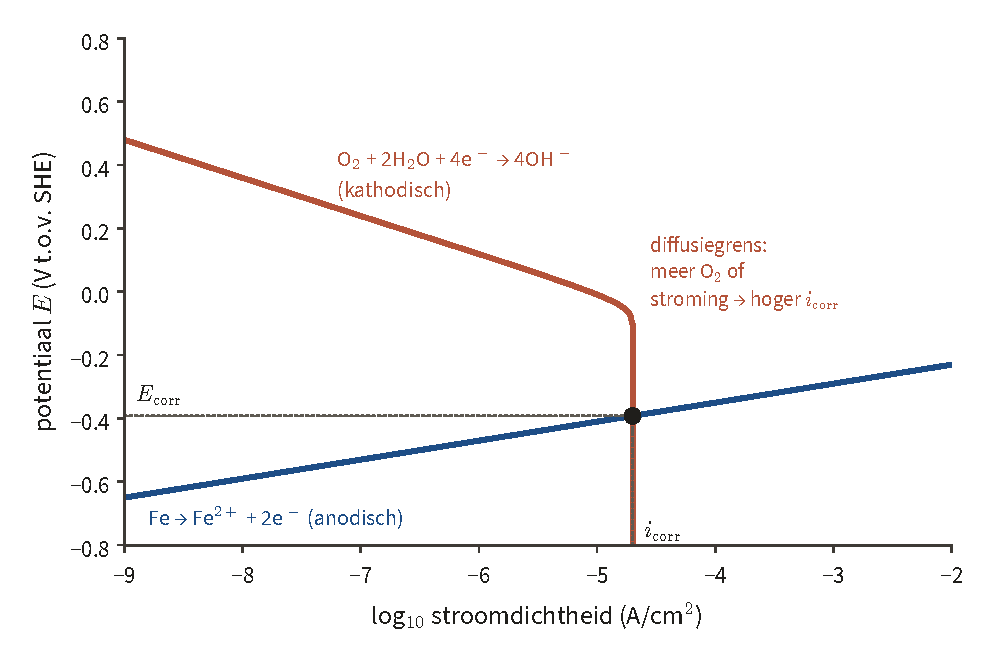
\includegraphics[width=0.75\linewidth]{Figuren/evans_diagram}
    \caption{Evansdiagram van staal in belucht water (schematisch). Het snijpunt van de anodische en de kathodische lijn bepaalt de corrosiepotentiaal en de corrosiestroom. Hier wordt de kathodische stroom begrensd door de aanvoer van zuurstof.}
    \label{fig:evans}
\end{figure}

Het Evansdiagram verklaart enkele vaststellingen uit de praktijk:
\begin{itemize}
\item In neutraal water is de aanvoer van opgeloste zuurstof meestal de traagste stap. Meer zuurstof, hogere temperatuur of sterkere stroming verschuift de diffusiegrens naar rechts en verhoogt $i_\mathrm{corr}$. Ontgassen van ketelvoedingswater (hoofdstuk~\ref{ch:niet-reagerend}) haalt precies die kathodische reactie weg.
\item Twee verschillende metalen in contact vormen een \emph{galvanisch koppel}: het minst edele metaal wordt anode. De verhouding van de oppervlakken telt: een kleine anode tegenover een grote kathode concentreert de volledige kathodische stroom op een klein stuk metaal. Stalen klinknagels in een koperen plaat zijn dus een slecht idee, koperen klinknagels in een stalen plaat veel minder.
\item Een opofferingsanode (zink, magnesium) of een uitwendige stroombron verschuift de potentiaal van het staal naar beneden, tot onder de evenwichtspotentiaal van ijzer: de anodische stroom van het staal valt weg (\S~\ref{sec:sturen-stabiliteit}).
\end{itemize}

\subsection{Het Pourbaix-diagram}
\label{sec:pourbaix}

Het \emph{Pourbaix-diagram} is het fasediagram van de elektrochemie. Waar een gewoon fasediagram (\S~\ref{sec:fasediagram}) de stabiele fase toont in functie van $T$ en $p$, toont een Pourbaix-diagram de stabiele vorm van een element in functie van de potentiaal $E$ (de oxiderende kracht van de omgeving) en de pH (want veel reacties verbruiken H$^+$ of OH$^-$). Het verdeelt het vlak in drie soorten gebieden:
\begin{itemize}
\item \textbf{immuniteit}: het metaal zelf is stabiel;
\item \textbf{corrosie}: opgeloste ionen zijn stabieler, het metaal lost op;
\item \textbf{passiviteit}: een vast oxide of hydroxide is stabiel en kan het metaal afschermen.
\end{itemize}
Op elke grenslijn hebben de twee soorten dezelfde Gibbs-energie. Reacties met enkel elektronen geven horizontale lijnen, reacties met enkel H$^+$ verticale, en reacties met beide schuine lijnen, waarvan Nernst de helling geeft.

\subsubsection{Het stabiliteitsgebied van water: afleiding van de grenslijnen}
\label{sec:pourbaix-waterlijnen}

Vrijwel alle Pourbaix-diagrammen bevatten twee schuine lijnen die het stabiliteitsgebied van water begrenzen. Buiten deze grenzen is vloeibaar water thermodynamisch niet stabiel. We leiden beide lijnen expliciet af met de vergelijking van Nernst (vergelijking~\eqref{eq:nernst}).

\textbf{Bovengrens: oxidatie van water tot zuurstof.} Bij hoge potentiaal wordt water geoxideerd:
\[
\mathrm{2\,H_2O \rightleftharpoons O_2 + 4\,H^+ + 4\,e^-}, \qquad E^\circ=\SI{1.23}{\volt}\ (n=4).
\]
Met $a_{\mathrm{H_2O}}\approx1$ en, als referentie, $p_{\mathrm{O_2}}=\SI{1}{\bar}$, is het reactiequoti\"ent voor de \emph{reductie}-vorm $Q=1/a_{\mathrm{H^+}}^4$. De Nernstvergelijking geeft:
\[
E = E^\circ - \frac{RT}{4F}\ln\frac{1}{a_{\mathrm{H^+}}^4} = E^\circ + \frac{RT}{F}\ln a_{\mathrm{H^+}}.
\]
Met $\ln a_{\mathrm{H^+}} = -\ln(10)\cdot\mathrm{pH}$ en $RT\ln(10)/F=\SI{0.0592}{\volt}$ bij \SI{298}{\kelvin} (\S~\ref{sec:nernst-elektrochemie}):
\begin{equation}
\boxed{\;E_{\mathrm{O_2/H_2O}} = \SI{1.23}{\volt} - \num{0.0592}\cdot\mathrm{pH}.\;}
\label{eq:lijn-boven}
\end{equation}

\textbf{Ondergrens: reductie van water tot waterstof.} Bij lage potentiaal wordt water (via $\mathrm{H^+}$) gereduceerd tot waterstofgas:
\[
\mathrm{2\,H^+ + 2\,e^- \rightleftharpoons H_2}, \qquad E^\circ=\SI{0}{\volt}\ (n=2).
\]
Met $p_{\mathrm{H_2}}=\SI{1}{\bar}$ als referentie is $Q=1/a_{\mathrm{H^+}}^2$, zodat op dezelfde manier:
\begin{equation}
\boxed{\;E_{\mathrm{H^+/H_2}} = 0 - \num{0.0592}\cdot\mathrm{pH}.\;}
\label{eq:lijn-onder}
\end{equation}

Beide lijnen dalen met \SI{0.0592}{\volt} per pH-eenheid en blijven \SI{1.23}{\volt} uit elkaar (figuur~\ref{fig:pourbaix-generiek}). Bij pH~7 ligt de bovengrens op \SI{0.82}{\volt}, de ondergrens op \SI{-0.41}{\volt}. Daartussen is water stabiel; erboven ontwikkelt het zuurstof, eronder waterstof. Bijna alle corrosie in de praktijk speelt zich tussen die twee lijnen af.

\begin{figure}[htb]
    \centering
    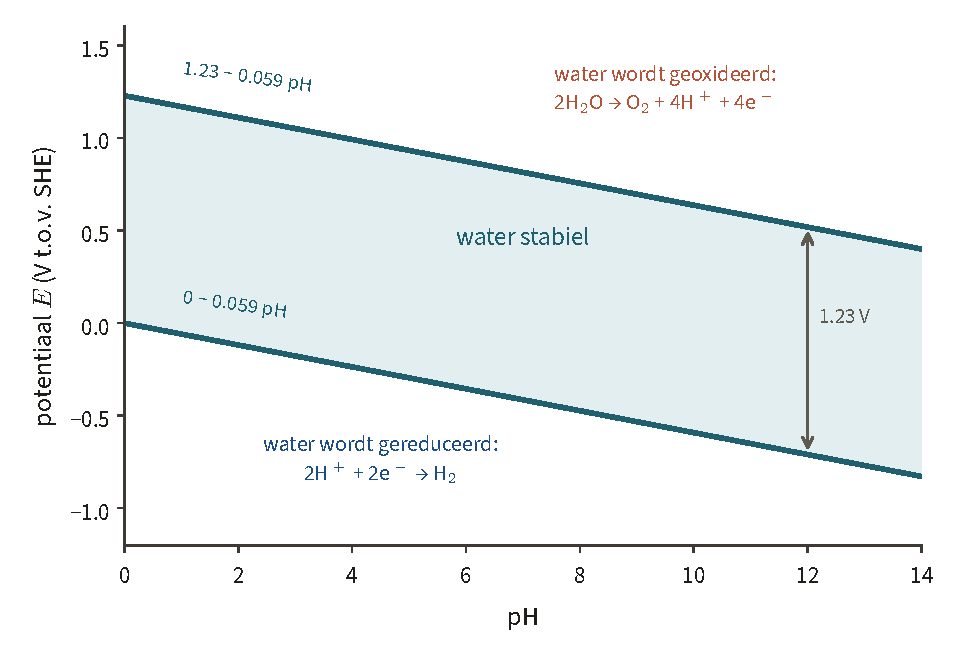
\includegraphics[width=0.75\linewidth]{Figuren/pourbaix_water}
    \caption{Het stabiliteitsgebied van water. Beide grenslijnen dalen met \SI{0.0592}{\volt} per pH-eenheid en liggen altijd \SI{1.23}{\volt} uit elkaar. In de volgende Pourbaix-diagrammen zijn ze als stippellijnen ingetekend.}
    \label{fig:pourbaix-generiek}
\end{figure}

\subsection{Zelf een Pourbaix-diagram opstellen: zink}
\label{sec:pourbaix-zelf}

Een Pourbaix-diagram is geen mysterie: het volgt volledig uit tabelwaarden van $\Delta_fG^\circ$ en de vergelijking van Nernst. We stellen het diagram van zink stap voor stap op.

\paragraph{Stap 1: kies de soorten en zoek $\Delta_fG^\circ$.} We beperken ons tot de vier belangrijkste vormen van zink in water (waarden in kJ/mol bij \SI{298}{\kelvin}, uit de NBS-tabellen):
\begin{center}
\begin{tabular}{lcccc}
\toprule
soort & Zn(s) & Zn$^{2+}$(aq) & Zn(OH)$_2$(s) & ZnO$_2^{2-}$(aq) \\
$\Delta_fG^\circ$ & 0 & $-147.1$ & $-553.5$ & $-384.2$ \\
\bottomrule
\end{tabular}
\end{center}
Daarnaast is $\Delta_fG^\circ(\mathrm{H_2O,l}) = \SI{-237.1}{\kilo\joule\per\mole}$ en $\Delta_fG^\circ(\mathrm{H^+}) = 0$.

\paragraph{Stap 2: kies de activiteit van de opgeloste ionen.} Bij corrosie stelt men de grens meestal bij $a = 10^{-6}$: lost er minder dan dat op, dan noemt men het metaal praktisch niet aangetast.

\paragraph{Stap 3: schrijf elke grensreactie en pas Nernst toe.} Elke grens is een evenwicht tussen twee soorten. Er zijn drie types.

\emph{Horizontale lijn, enkel elektronen.} $\mathrm{Zn^{2+} + 2\,e^- \rightleftharpoons Zn}$ met $E^\circ = \Delta_fG^\circ(\mathrm{Zn^{2+}})/2F = \SI{-0.762}{\volt}$:
\[
E = -0.762 + \frac{0.0592}{2}\log a_{\mathrm{Zn^{2+}}} = -0.762 - 0.178 = \SI{-0.94}{\volt}.
\]

\emph{Verticale lijn, enkel H$^+$.} $\mathrm{Zn(OH)_2 + 2\,H^+ \rightleftharpoons Zn^{2+} + 2\,H_2O}$ heeft $\Delta_rG^\circ = -147.1 + 2(-237.1) - (-553.5) = \SI{-67.8}{\kilo\joule\per\mole}$, dus $\log K = 67\,800/(2.303\,RT) = 11.9$. Met $K = a_{\mathrm{Zn^{2+}}}/a_{\mathrm{H^+}}^2$ volgt $\log a_{\mathrm{Zn^{2+}}} = 11.9 - 2\,\mathrm{pH}$, en de grens $a = 10^{-6}$ ligt bij pH~8.9. Op dezelfde manier ligt de grens Zn(OH)$_2$/ZnO$_2^{2-}$ bij pH~11.8.

\emph{Schuine lijn, elektronen en H$^+$.} $\mathrm{Zn(OH)_2 + 2\,H^+ + 2\,e^- \rightleftharpoons Zn + 2\,H_2O}$ heeft $\Delta_rG^\circ = 2(-237.1) - (-553.5) = \SI{79.2}{\kilo\joule\per\mole}$, dus $E^\circ = -79\,200/2F = \SI{-0.41}{\volt}$ en
\[
E = -0.41 - 0.0592\,\mathrm{pH}.
\]
Per H$^+$ per elektron daalt de lijn met \SI{0.0592}{\volt} per pH-eenheid, net als de waterlijnen.

\paragraph{Stap 4: teken en controleer.} De lijnen snijden elkaar; van elke lijn houd je enkel het stuk waar beide soorten ook echt de stabielste zijn. Figuur~\ref{fig:pourbaix-zink} toont het resultaat. Een rekenblad kan hetzelfde zonder lijnen te zoeken: bereken voor elk punt $(E, \mathrm{pH})$ de Gibbsenergie van elke soort ten opzichte van het metaal en kleur het punt volgens de laagste waarde. Zo zijn alle diagrammen in dit hoofdstuk berekend.

\begin{figure}[htb]
    \centering
    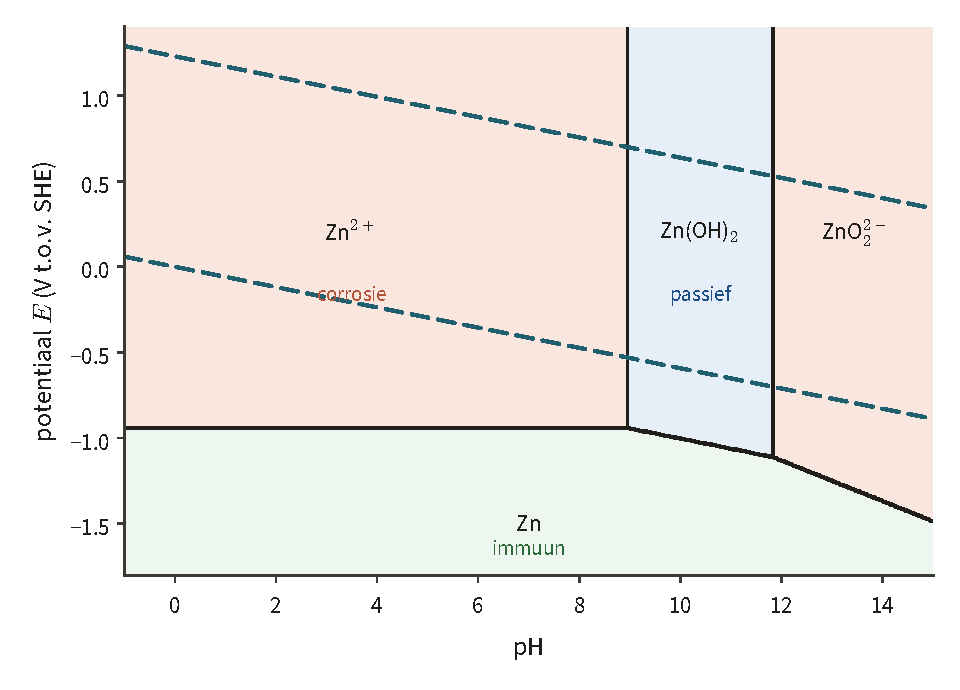
\includegraphics[width=0.75\linewidth]{Figuren/pourbaix_zink}
    \caption{Pourbaix-diagram van zink bij \SI{25}{\celsius} en ionactiviteit $10^{-6}$ (berekend uit NBS-gegevens). Rood: corrosie, blauw: passief, groen: immuun. Stippellijnen: stabiliteitsgebied van water.}
    \label{fig:pourbaix-zink}
\end{figure}

\begin{toepassing}{Waarom verzinkt staal zo goed werkt}
Zink is \emph{amfoteer}: het lost op in zuur (Zn$^{2+}$) en in sterke base (ZnO$_2^{2-}$), maar tussen pH~9 en~12 vormt het een beschermende hydroxide- en carbonaatlaag. In regenwater en de meeste natuurlijke milieus ligt de pH daar niet ver vandaan, zodat een zinklaag maar traag verdwijnt (enkele \si{\micro\metre} per jaar). Raakt de laag beschadigd, dan wordt het blootgestelde staal kathodisch beschermd: zink ligt in het diagram veel lager dan ijzer en offert zich op. Daarom is verzinken (thermisch of galvanisch) de goedkoopste duurzame bescherming voor vangrails, bouwstaal en elektriciteitsmasten. In beton (pH~13) of in contact met kalk werkt zink veel minder goed, wat het diagram ook toont.
\end{toepassing}

\subsection{Het Pourbaix-diagram van ijzer}
\label{sec:pourbaix-ijzer}

Het diagram van ijzer (figuur~\ref{fig:pourbaix-ijzer}) toont:

\begin{itemize}
\item Bij lage potentialen: immuniteit (metaal Fe stabiel), onder ongeveer \SI{-0.6}{\volt}.
\item Bij lage pH: corrosie, als opgelost $\mathrm{Fe^{2+}}$ of, bij hoge potentiaal, $\mathrm{Fe^{3+}}$.
\item Bij neutrale tot basische pH: passiviteit door de vaste oxiden magnetiet ($\mathrm{Fe_3O_4}$) en hematiet ($\mathrm{Fe_2O_3}$).
\end{itemize}
Een belangrijke vaststelling: de immuniteitsgrens van ijzer ligt bij elke pH \emph{onder} de onderste waterlijn. IJzer is dus nergens stabiel in contact met water. In zuur water (lage pH, lage potentiaal) corrodeert het zelfs zonder zuurstof, met H$^+$ als oxidator en waterstofgas als product.

\begin{figure}[htb]
    \centering
    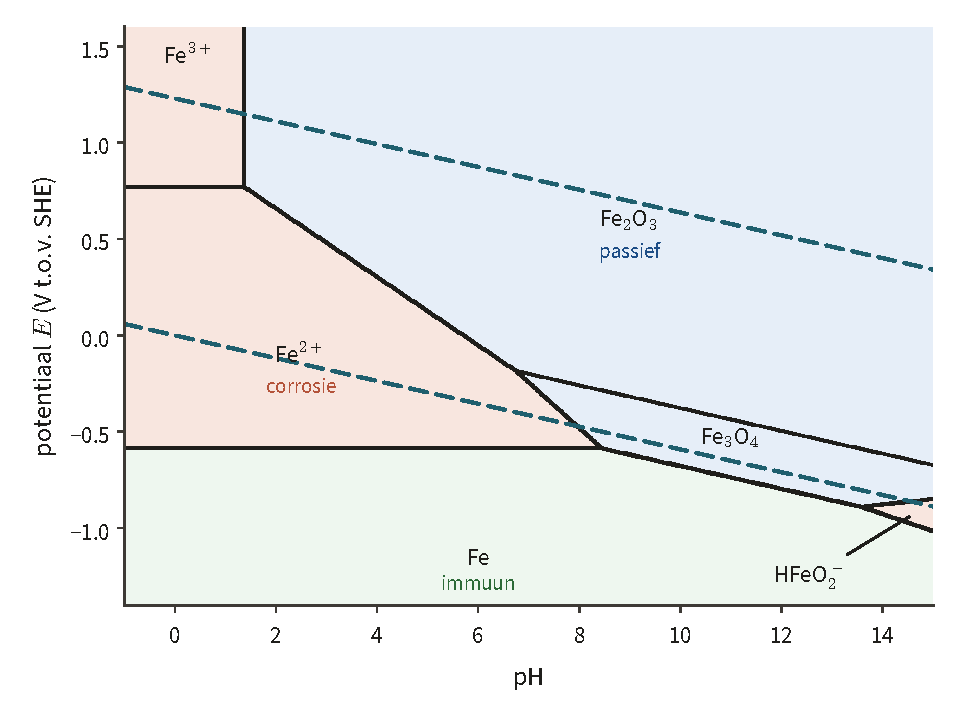
\includegraphics[width=0.75\linewidth]{Figuren/pourbaix_ijzer}
    \caption{Pourbaix-diagram van ijzer bij \SI{25}{\celsius} en ionactiviteit $10^{-6}$ (berekend uit NBS-gegevens; Fe(OH)$_2$ en FeOOH zijn weggelaten). Bij neutrale pH en beluchting (bovenaan het watergebied) ligt ijzer in het gebied van Fe$_2$O$_3$; zonder lucht (onderaan) in dat van Fe$^{2+}$ of Fe$_3$O$_4$.}
    \label{fig:pourbaix-ijzer}
\end{figure}

Het diagram voorspelt dat ijzer in belucht neutraal water passief zou zijn. Toch roest een stalen balk. IJzeroxiden zijn echter poreus en weinig hechtend, zodat de bescherming onvolledig is; bovendien verschuiven chloride-ionen de grenzen in het nadeel van de passieve laag. Daarom wordt staal gecoat, geverfd of gelegeerd met chroom (roestvast staal), dat een veel compactere oxidefilm vormt.

\section{Materiaalkeuze en corrosiebeheersing}

\subsection{Materiaalkeuze op basis van Pourbaix-diagrammen}
\label{sec:materiaalkeuze}

Een Pourbaix-diagram zegt welke toestand stabiel is, niet hoe snel die bereikt wordt. Een metaal in het corrosiegebied kan praktisch onaangetast blijven als de reactie traag is; een metaal in het passieve gebied kan toch corroderen als de oxidefilm lokaal beschadigd raakt. Materiaalkeuze combineert dus altijd thermodynamica en kinetiek.

\begin{voorbeeld}{Aluminium: thermodynamisch reactief, praktisch inert}
Aluminium bezit een sterk negatieve standaardpotentiaal ($E^\circ = \SI{-1.66}{\volt}$, tabel~\ref{tab:reductiepotentialen}), wat erop wijst dat oxidatie thermodynamisch zeer gunstig is. Toch behoort aluminium tot de meest corrosiebestendige constructiematerialen. De verklaring ligt in de vorming van een uiterst dunne, compacte en sterk hechtende laag aluminiumoxide, die het onderliggende metaal afschermt van de omgeving. Figuur~\ref{fig:pourbaix-al-cu} toont dat aluminium enkel passief is tussen pH~4.5 en~9. Daarbuiten lost het oxide op: in zuur als Al$^{3+}$, in base als aluminaat Al(OH)$_4^-$. Daarom mag een aluminium pan niet in de vaatwasmachine met een sterk alkalisch vaatwasmiddel, en ontkalkt men aluminium niet met sterk zuur.
\end{voorbeeld}

\begin{figure}[htb]
    \centering
    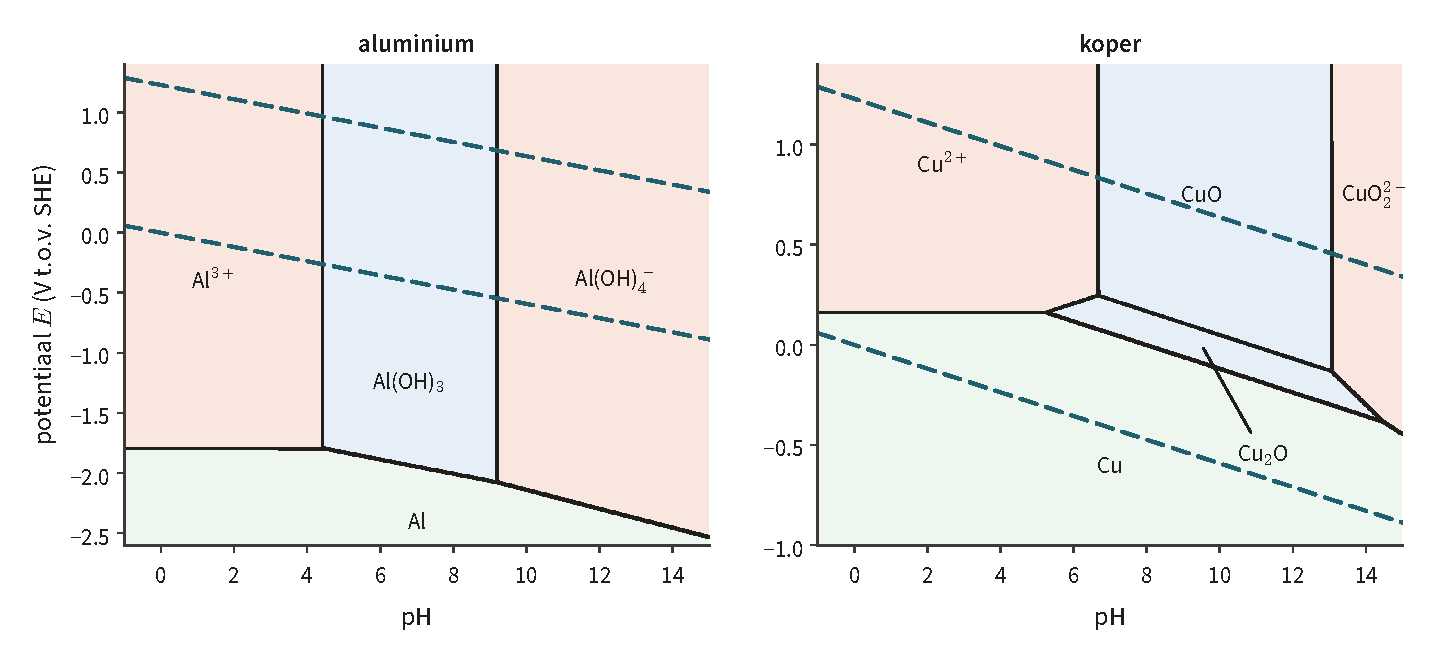
\includegraphics[width=\linewidth]{Figuren/pourbaix_al_cu}
    \caption{Pourbaix-diagrammen van aluminium (links) en koper (rechts) bij \SI{25}{\celsius} en ionactiviteit $10^{-6}$ (berekend uit NBS-gegevens). Let op de verschillende schaal van de potentiaalas.}
    \label{fig:pourbaix-al-cu}
\end{figure}

\begin{voorbeeld}{Koper: een edel metaal in zuur zonder lucht}
Bij koper ligt het immuniteitsgebied grotendeels \emph{boven} de onderste waterlijn (figuur~\ref{fig:pourbaix-al-cu}). In zuur water zonder opgeloste zuurstof is H$^+$ dus niet sterk genoeg om koper te oxideren: koper lost niet op in verdund zoutzuur, zink en ijzer wel. Met lucht erbij verschuift de potentiaal naar boven en komt koper in het Cu$^{2+}$-gebied terecht; daarom corrodeert koper wel in belucht zuur. Bij neutrale pH vormt koper een laagje Cu$_2$O en, buiten, op termijn het groene patina. Koperen waterleidingen gaan zo decennia mee, tenzij het water zuur en zuurstofrijk is.
\end{voorbeeld}

\begin{voorbeeld}{Roestvast staal}
Roestvast staal bevat minstens \SI{12}{\percent} chroom. Chroom vormt een compacte oxidefilm ($\mathrm{Cr_2O_3}$) die het onderliggende staal afschermt. Volgens het Pourbaix-diagram bevindt chroom zich in een groot passiviteitsgebied, terwijl de kinetiek van de oxidevorming uiterst gunstig is. De combinatie van beide eigenschappen leidt tot de uitstekende corrosieweerstand die roestvast staal kenmerkt.
\end{voorbeeld}

\subsection{Het sturen van thermodynamische stabiliteit}
\label{sec:sturen-stabiliteit}

Door de procesomstandigheden te wijzigen kan de ingenieur het werkpunt in het Pourbaix-diagram doelgericht verschuiven.

\begin{itemize}
\item \textbf{pH-wijziging}: toevoegen van zuur of base verschuift het punt horizontaal. Voor vele metalen leidt een verhoging van de pH tot passiviteit.
\item \textbf{Potentiaalwijziging}: een uitwendige spanning (kathodische bescherming) verschuift het punt verticaal naar het immuniteitsgebied.
\item \textbf{Legeren}: toevoegen van chroom, nikkel of molybdeen verandert het Pourbaix-diagram zelf.
\item \textbf{Inhibitors}: stoffen die de oxidefilm versterken of de corrosiekinetiek vertragen.
\end{itemize}

\begin{toepassing}{Kathodische bescherming van ondergrondse leidingen}
Aardgasleidingen en opslagtanks worden vaak kathodisch beschermd door een kleine gelijkstroom aan te leggen tussen het te beschermen staal en een ``opofferingsanode'' (magnesium of zink). Hierdoor wordt het staal tot een potentiaal gedwongen waar het zich in het immuniteitsgebied van zijn Pourbaix-diagram bevindt. De anode corrodeert langzaam en moet periodiek worden vervangen, maar de dure leiding blijft gespaard.
\end{toepassing}

\section{Samenvatting en reflectie}

Batterijen, brandstofcellen, elektrolysers en corrosie lijken verschillende werelden, maar ze steunen op dezelfde thermodynamica: $\Delta_rG = -nFE$ verbindt de spanning met de Gibbsenergie van hoofdstuk~\ref{ch:spontaniteit} en het evenwicht van hoofdstuk~\ref{ch:reagerend}. Of je nu groene waterstof produceert, een batterij kiest of een leiding beschermt, je stelt telkens dezelfde vragen: welke spanning laat de thermodynamica toe, hoeveel lading is nodig (Faraday), en hoeveel gaat verloren aan kinetiek? In het volgende hoofdstuk kijken we naar wat er aan oppervlakken gebeurt, waar ook de elektrodereacties plaatsvinden.

\begin{samenvatting}{Elektrochemische thermodynamica}
\begin{itemize}
\item De maximale niet-expansiearbeid is $-\Delta G$; in een cel wordt die elektrische arbeid: $\Delta_rG = -nFE$ en $\Delta_rG^\circ = -nFE^\circ = -RT\ln K$.
\item $E^\circ_\mathrm{cel} = E^\circ_\mathrm{kathode} - E^\circ_\mathrm{anode}$, met reductiepotentialen ten opzichte van de SHE.
\item Nernst: $E = E^\circ - (RT/nF)\ln Q$; bij \SI{298}{\kelvin} \SI{0.0592}{\volt}/$n$ per decade.
\item $(\partial E^\circ/\partial T)_p$ geeft $\Delta_rS^\circ$, en daarmee $\Delta_rH^\circ$, zonder calorimetrie.
\item Faraday: $m = ItM/nF$; energie per kg product $nFU/(M\eta_F)$. Water splitsen vraagt minstens \SI{1.23}{\volt} (omkeerbaar) en \SI{1.48}{\volt} zonder warmtetoevoer (thermoneutraal).
\item Overspanning (activering, ohmse verliezen, diffusie) maakt een elektrolyser duurder en een batterij zwakker. Tafel: $\eta = b\log(i/i_0)$; een katalysator verhoogt $i_0$.
\item Corrosie is een galvanische cel op \'e\'en metaal. De snelheid volgt uit $i_\mathrm{corr}$ via Faraday: \SI{1}{\micro\ampere\per\centi\metre\squared} $\approx$ \SI{12}{\micro\metre} staal per jaar.
\item Een Pourbaix-diagram toont de stabielste vorm als functie van $E$ en pH: immuniteit, corrosie, passiviteit. Het volgt volledig uit $\Delta_fG^\circ$ en Nernst, maar zegt niets over snelheid.
\end{itemize}
\end{samenvatting}

\begin{reflectie}{Elektrochemische thermodynamica}
\begin{enumerate}
\item Waarom kan een brandstofcel in principe een hoger rendement halen dan een verbrandingsmotor die dezelfde waterstof verbrandt?
\item Een batterij van \SI{1.5}{\volt} en een van \SI{3.7}{\volt} leveren dezelfde lading. Welke levert meer energie, en waarom?
\item Waarom stijgt het elektriciteitsverbruik van een elektrolyser als je hem harder laat werken (meer kilogram per uur)?
\item Hoe kan een elektrolyser warmte uit de omgeving opnemen? Onder welke spanning gebeurt dat?
\item Waarom is het ontgassen van ketelvoedingswater een corrosiebeschermingsmaatregel?
\item Waarom is een kleine stalen bout in een grote koperen plaat gevaarlijker dan het omgekeerde?
\item Aluminium heeft een veel negatievere standaardpotentiaal dan ijzer. Waarom roest een aluminium fietskader dan niet weg?
\item Een Pourbaix-diagram voorspelt dat ijzer in belucht neutraal water passief is. Waarom roest het toch?
\end{enumerate}
\end{reflectie}

\newpage
\section{Oefeningen}

% Oefeningen bij dit hoofdstuk (ingevoegd achteraan het hoofdstuk met \input).
% Een oefening:  \begin{oefening}[titel] ... \end{oefening}   (boek en website)
% De oplossing:  \begin{oplossing} ... \end{oplossing}       (enkel website, dichtgeklapt)

Neem $F = \SI{96485}{\coulomb\per\mole}$, $R = \SI{8.314}{\joule\per\mole\per\kelvin}$, $RT\ln 10/F = \SI{0.0592}{\volt}$ bij \SI{298}{\kelvin} en de standaardreductiepotentialen uit tabel~\ref{tab:reductiepotentialen}.

\begin{oefening}[De Daniell-cel buiten standaardomstandigheden]
Voor de Daniell-cel \(\mathrm{Zn(s) + Cu^{2+}(aq) \rightarrow Zn^{2+}(aq) + Cu(s)}\) geldt \(E^\circ = 1.10\,\mathrm{V}\).

\begin{enumerate}
\item[(a)]
  Bereken \(\Delta_r G^\circ\) en de evenwichtsconstante \(K\) bij \(298\,\mathrm{K}\). Wat betekent die waarde voor de \(\mathrm{Cu^{2+}}\)-concentratie in een volledig ontladen cel?
\item[(b)]
  Bereken de celspanning wanneer \(c_{\mathrm{Zn^{2+}}} = 0.10\,\mathrm{mol/L}\) en \(c_{\mathrm{Cu^{2+}}} = 1.0\,\mathrm{mol/L}\).
\item[(c)]
  Hoe verandert de spanning wanneer beide concentraties gehalveerd worden? En wanneer je ze omwisselt?
\item[(d)]
  Waarom is de spanning van een batterij tijdens het grootste deel van de ontlading vrijwel constant?
\end{enumerate}
\end{oefening}
\begin{oplossing}
\textbf{Resultaat:} (a) \(\Delta_r G^\circ\) = \textbf{\ensuremath{-}212 kJ/mol}, \(K\) \ensuremath{\approx{}} \textbf{1.5\ensuremath{\cdot{}}10\ensuremath{^{37}}}. (b) \(E\) = \textbf{1.13 V}. (c) Halveren: \textbf{geen verandering}; omwisselen: \textbf{1.07 V}. (d) \(E\) hangt slechts \textbf{logaritmisch} af van de concentraties.

\textbf{(a)} \(\Delta_r G^\circ = -nFE^\circ = -(2)(96485)(1.10) = -212.3\,\mathrm{kJ/mol}\) en

\[
\ln K = \frac{nFE^\circ}{RT} = \frac{(2)(96485)(1.10)}{(8.314)(298.15)} = 85.6 \quad\Rightarrow\quad K = 1.5\times10^{37}
\]

In evenwicht is \(c_{\mathrm{Zn^{2+}}}/c_{\mathrm{Cu^{2+}}} = 10^{37}\): een `lege' Daniell-cel bevat praktisch geen \(\mathrm{Cu^{2+}}\) meer. De cel stopt omdat de koperionen op zijn, niet omdat het evenwicht halverwege ligt.

\textbf{(b)} Met \(Q = c_{\mathrm{Zn^{2+}}}/c_{\mathrm{Cu^{2+}}}\) (vaste metalen hebben activiteit 1):

\[
E = 1.10 - \frac{0.0592}{2}\log_{10}\frac{0.10}{1.0} = 1.10 + 0.0296 = 1.13\,\mathrm{V}
\]

\textbf{(c)} Halveren van beide concentraties laat \(Q\) ongewijzigd: \(E = 1.13\,\mathrm{V}\). Omwisselen geeft \(Q = 10\) en \(E = 1.10 - 0.0296 = 1.07\,\mathrm{V}\).

\textbf{(d)} Een factor tien in \(Q\) verandert de spanning slechts met \(29.6\,\mathrm{mV}\) (voor \(n = 2\)). Pas helemaal op het einde van de ontlading, wanneer een reactant bijna op is en \(Q\) met vele grootteordes verandert, zakt de spanning snel in. Batterijen met vaste reactanten (zoals de loodaccu of Li-ion) hebben bovendien activiteiten die bijna constant blijven.
\end{oplossing}

\begin{oefening}[Chloor en natronloog uit zout water]
In de chlooralkali-elektrolyse wordt pekel ontleed. Aan de anode ontstaat chloor (\(\mathrm{2\,Cl^- \rightarrow Cl_2 + 2\,e^-}\)), aan de kathode waterstof en hydroxide (\(\mathrm{2\,H_2O + 2\,e^- \rightarrow H_2 + 2\,OH^-}\), met \(E = -0.83\,\mathrm{V}\) bij pH 14). Chloor is de grondstof voor PVC en voor bleekwater.

\begin{enumerate}
\item[(a)]
  Bereken de thermodynamische minimumspanning met \(E^\circ(\mathrm{Cl_2/Cl^-}) = 1.36\,\mathrm{V}\).
\item[(b)]
  Een industriële membraancel werkt bij \(3.2\,\mathrm{V}\). Bereken het elektriciteitsverbruik per ton chloor (\(M = 70.90\,\mathrm{g/mol}\)).
\item[(c)]
  Welk deel van die energie is thermodynamisch noodzakelijk? Waar gaat de rest naartoe?
\end{enumerate}
\end{oefening}
\begin{oplossing}
\textbf{Resultaat:} (a) \(E_{\min}\) = \textbf{2.19 V}. (b) Ongeveer \textbf{2420 kWh per ton Cl\ensuremath{_{2}}}. (c) \textbf{68 \%} (2.19/3.2); de rest wordt \textbf{warmte} door overspanning en ohmse weerstand.

\textbf{(a)} De cel moet de reactie \(\mathrm{2\,Cl^- + 2\,H_2O \rightarrow Cl_2 + H_2 + 2\,OH^-}\) afdwingen. De omkeerbare celspanning is \(E = E_{\text{kathode}} - E_{\text{anode}} = -0.83 - 1.36 = -2.19\,\mathrm{V}\), dus minstens \(2.19\,\mathrm{V}\) moet worden aangelegd.

\textbf{(b)} Een ton chloor is \(10^6/70.90 = 1.41\times10^{4}\,\mathrm{mol}\), met telkens 2 mol elektronen per mol \(\mathrm{Cl_2}\):

\[
Q = (2)(1.41\times10^{4})(96485) = 2.72\times10^{9}\,\mathrm{C}, \qquad W = QV = (2.72\times10^{9})(3.2) = 8.7\times10^{9}\,\mathrm{J} = 2420\,\mathrm{kWh}
\]

\textbf{(c)} Bij \(2.19\,\mathrm{V}\) zou \(1660\,\mathrm{kWh}\) volstaan, dus \(68\,\%\) van het verbruik is thermodynamisch onvermijdelijk. De rest (\(1.0\,\mathrm{V}\)) gaat verloren als warmte: overspanning aan de elektroden (kinetiek), weerstand van de elektrolyt en het membraan. De chlooralkali-industrie is een van de grootste elektriciteitsverbruikers in de Belgische chemie (onder meer in Antwerpen en Tessenderlo).
\end{oplossing}

\begin{oefening}[Brandstofcel of verbrandingsmotor?]
Een PEM-brandstofcel zet waterstof om in vloeibaar water: \(\mathrm{H_2(g) + \tfrac{1}{2}\,O_2(g) \rightarrow H_2O(l)}\), met \(\Delta_r H^\circ = -285.8\,\mathrm{kJ/mol}\) en \(\Delta_r G^\circ = -237.1\,\mathrm{kJ/mol}\) bij \(298\,\mathrm{K}\).

\begin{enumerate}
\item[(a)]
  Bereken de maximale elektrische arbeid per mol \(\mathrm{H_2}\) en de standaardcelpotentiaal.
\item[(b)]
  Een cel werkt bij \(0.70\,\mathrm{V}\). Bereken de geleverde elektrische arbeid per mol \(\mathrm{H_2}\), het rendement ten opzichte van \(\Delta_r G^\circ\) en ten opzichte van \(\Delta_r H^\circ\), en de warmte die per mol vrijkomt.
\item[(c)]
  Vergelijk met het Carnot-rendement van een warmtemotor die werkt tussen \(900\,\mathrm{K}\) en \(300\,\mathrm{K}\) (hoofdstuk 3). Waarom geldt de Carnot-grens niet voor een brandstofcel?
\item[(d)]
  Hoeveel cellen in serie zijn nodig voor een stapel die \(280\,\mathrm{V}\) levert, zoals in een waterstofauto?
\end{enumerate}
\end{oefening}
\begin{oplossing}
\textbf{Resultaat:} (a) \(w_{\max}\) = \textbf{237 kJ/mol}, \(E^\circ\) = \textbf{1.23 V}. (b) \textbf{135 kJ/mol}; rendement \textbf{57 \%} (t.o.v. \(\Delta G\)) of \textbf{47 \%} (t.o.v. \(\Delta H\)); \textbf{151 kJ/mol} warmte. (c) Carnot: \textbf{67 \%}, maar een brandstofcel is geen warmtemotor. (d) \textbf{400 cellen}.

\textbf{(a)} \(w_{\max} = -\Delta_r G^\circ = 237.1\,\mathrm{kJ/mol}\) en \(E^\circ = 237\,100/(2 \times 96485) = 1.23\,\mathrm{V}\).

\textbf{(b)} \(w = nFE = (2)(96485)(0.70) = 135\,\mathrm{kJ/mol}\). Rendement: \(0.70/1.23 = 57\,\%\) ten opzichte van de maximale arbeid, of \(135/285.8 = 47\,\%\) ten opzichte van de verbrandingswarmte (de gebruikelijke definitie bij voertuigen). De energiebalans (eerste hoofdwet) geeft de warmte: \(285.8 - 135 = 151\,\mathrm{kJ/mol}\), die met koelwater afgevoerd wordt.

\textbf{(c)} \(\eta_{\text{Carnot}} = 1 - 300/900 = 67\,\%\); echte automotoren halen \(25\)--\(35\,\%\). Een warmtemotor zet chemische energie eerst om in warmte bij hoge temperatuur en moet dan een deel daarvan afgeven aan de koude omgeving; daaruit volgt de Carnot-grens. Een brandstofcel zet de Gibbs-energie rechtstreeks om in elektrische arbeid, zonder tussenstap via warmte: de enige grens is \(-\Delta_r G\) (vergelijking 7.5). Het theoretisch maximum is \(237/286 = 83\,\%\), onafhankelijk van een temperatuurverschil.

\textbf{(d)} \(280/0.70 = 400\) cellen in serie. De stroom (en dus het vermogen) bepaalt men met het celoppervlak.
\end{oplossing}

\begin{oefening}[Hoeveel lithium zit er in je smartphone?]
Een smartphonebatterij heeft een capaciteit van \(4000\,\mathrm{mAh}\) bij een gemiddelde spanning van \(3.85\,\mathrm{V}\). Bij het ontladen verhuist lithium als \(\mathrm{Li^+}\) van de grafietelektrode (\(\mathrm{LiC_6}\)) naar de kathode, met één elektron per lithiumatoom.

\begin{enumerate}
\item[(a)]
  Bereken de opgeslagen energie in Wh en in kJ. Vergelijk met de energie in een reep chocolade van \(100\,\mathrm{g}\) (ongeveer \(2200\,\mathrm{kJ}\)).
\item[(b)]
  Hoeveel mol elektronen worden tijdens een volledige ontlading uitgewisseld?
\item[(c)]
  Hoeveel gram lithium moet minstens verhuizen, en hoeveel gram grafiet is nodig om het op te slaan?
\item[(d)]
  Waarom gebruikt men lithium en geen natrium of zink in een batterij voor een smartphone? Gebruik tabel 7.1.
\end{enumerate}
\end{oefening}
\begin{oplossing}
\textbf{Resultaat:} (a) \textbf{15.4 Wh} = 55 kJ, ongeveer \textbf{40 keer minder} dan een reep chocolade. (b) \textbf{0.149 mol} elektronen. (c) \textbf{1.04 g Li} en \textbf{10.8 g grafiet}. (d) Lithium heeft de \textbf{meest negatieve} reductiepotentiaal en de kleinste molaire massa.

\textbf{(a)} \(E = (4.0\,\mathrm{Ah})(3.85\,\mathrm{V}) = 15.4\,\mathrm{Wh} = 15.4 \times 3600\,\mathrm{J} = 55\,\mathrm{kJ}\). Een reep chocolade bevat \(2200/55 = 40\) keer meer energie. Chemische energie in voedsel (verbranding met zuurstof uit de lucht) is veel geconcentreerder dan wat een batterij opslaat.

\textbf{(b)} \(Q = (4.0\,\mathrm{A})(3600\,\mathrm{s}) = 14\,400\,\mathrm{C}\), dus \(n_e = Q/F = 0.149\,\mathrm{mol}\).

\textbf{(c)} Eén elektron per Li: \(0.149\,\mathrm{mol}\) Li \(= (0.149)(6.94) = 1.04\,\mathrm{g}\). In \(\mathrm{LiC_6}\) horen bij elk Li zes koolstofatomen: \((6)(0.149)(12.01) = 10.8\,\mathrm{g}\) grafiet. Een echte batterij weegt ongeveer \(60\,\mathrm{g}\): de kathode, de elektrolyt, de stroomcollectoren en de behuizing wegen veel meer.

\textbf{(d)} Lithium heeft de meest negatieve standaardreductiepotentiaal (\(-3.04\,\mathrm{V}\), tabel 7.1): als anodemateriaal levert het de hoogste celspanning. Bovendien is het het lichtste metaal (\(6.94\,\mathrm{g/mol}\)), zodat het de meeste lading per gram levert. Natrium (\(-2.71\,\mathrm{V}\), \(23\,\mathrm{g/mol}\)) is goedkoper en wordt onderzocht voor stationaire opslag; zink (\(-0.76\,\mathrm{V}\)) geeft veel minder spanning.
\end{oplossing}

\begin{oefening}[De citroenbatterij]
In een klassiek schoolexperiment steek je een gegalvaniseerde (verzinkte) spijker en een koperen muntstuk in een citroen. Het citroensap heeft een pH van \(2.3\). Aan het koper worden waterstofionen gereduceerd (\(\mathrm{2\,H^+ + 2\,e^- \rightarrow H_2}\)); het koper zelf reageert niet.

\begin{enumerate}
\item[(a)]
  Schrijf de celreactie en bereken de standaardcelpotentiaal.
\item[(b)]
  Bereken de celspanning met \(c_{\mathrm{Zn^{2+}}} = 1\times10^{-4}\,\mathrm{mol/L}\) en \(p_{\mathrm{H_2}} = 1\,\mathrm{bar}\).
\item[(c)]
  Een rode led heeft minstens \(1.8\,\mathrm{V}\) nodig. Hoeveel citroenen moet je in serie schakelen? Waarom brandt de led toch nauwelijks?
\item[(d)]
  Waarom krijg je een veel kleinere spanning met twee koperen muntstukken?
\end{enumerate}
\end{oefening}
\begin{oplossing}
\textbf{Resultaat:} (a) \(\mathrm{Zn + 2\,H^+ \rightarrow Zn^{2+} + H_2}\), \(E^\circ\) = \textbf{0.76 V}. (b) \(E\) \ensuremath{\approx{}} \textbf{0.74 V}. (c) \textbf{3 citroenen}; de stroom is zeer klein door de grote inwendige weerstand en traagheid van de elektroden. (d) Twee gelijke elektroden geven \(E^\circ = 0\).

\textbf{(a)} Anode: \(\mathrm{Zn \rightarrow Zn^{2+} + 2\,e^-}\); kathode: \(\mathrm{2\,H^+ + 2\,e^- \rightarrow H_2}\). Samen: \(\mathrm{Zn + 2\,H^+ \rightarrow Zn^{2+} + H_2}\) met \(E^\circ = 0.00 - (-0.76) = 0.76\,\mathrm{V}\). Het koper dient enkel als geleidend oppervlak.

\textbf{(b)} Met \(a_{\mathrm{H^+}} = 10^{-2.3}\):

\[
E = 0.76 - \frac{0.0592}{2}\log_{10}\frac{c_{\mathrm{Zn^{2+}}}\,p_{\mathrm{H_2}}}{a_{\mathrm{H^+}}^2} = 0.76 - 0.0296\,(-4 + 4.6) = 0.74\,\mathrm{V}
\]

\textbf{(c)} \(1.8/0.74 = 2.4\), dus drie citroenen in serie (\(2.2\,\mathrm{V}\)). De thermodynamica geeft enkel de spanning bij nulstroom. Zodra er stroom loopt, verliest de cel spanning door de weerstand van het citroensap en door de trage waterstofvorming op koper (overspanning). De stroom blijft beperkt tot enkele tienden van een milliampère.

\textbf{(d)} Met twee identieke elektroden is \(E^\circ = 0\): enkel een klein concentratieverschil kan een spanning geven (zoals in de concentratiecel uit de theorie).
\end{oplossing}

\begin{oefening}[Roest ijzer ook zonder zuurstof? Het Pourbaix-diagram]
In een Pourbaix-diagram tekent men de grens tussen immuniteit en corrosie bij een conventionele ionactiviteit van \(10^{-6}\).

\begin{enumerate}
\item[(a)]
  Bereken de potentiaal van de horizontale lijn \(\mathrm{Fe^{2+} + 2\,e^- \rightleftharpoons Fe}\) bij \(a_{\mathrm{Fe^{2+}}} = 10^{-6}\). Waarom is deze lijn horizontaal?
\item[(b)]
  Vergelijk met de ondergrens van het stabiliteitsgebied van water bij pH 7. Kan ijzer in zuurstofvrij, neutraal water thermodynamisch oxideren onder vorming van waterstof? Bereken de celspanning.
\item[(c)]
  Waarom roest ijzer in zuurstofvrij water in de praktijk toch nauwelijks?
\item[(d)]
  Tot welke potentiaal moet een stalen pijpleiding minstens gebracht worden voor kathodische bescherming? Waarom is een zinkanode daarvoor geschikt?
\end{enumerate}
\end{oefening}
\begin{oplossing}
\textbf{Resultaat:} (a) \(E\) = \textbf{\ensuremath{-}0.62 V}, horizontaal want zonder H\ensuremath{^{+}}. (b) Waterlijn bij pH 7: \ensuremath{-}0.41 V; \(E_{\text{cel}}\) = \textbf{+0.20 V}: \textbf{ja}, thermodynamisch mogelijk. (c) De reactie is \textbf{kinetisch} zeer traag. (d) Onder \textbf{\ensuremath{-}0.62 V}; zink (\(-0.76\,\mathrm{V}\)) oxideert liever dan ijzer.

\textbf{(a)} Nernst voor de reductie, met \(Q = 1/a_{\mathrm{Fe^{2+}}}\):

\[
E = -0.44 - \frac{0.0592}{2}\log_{10}\frac{1}{10^{-6}} = -0.44 - 0.178 = -0.62\,\mathrm{V}
\]

Er komen geen \(\mathrm{H^+}\)- of \(\mathrm{OH^-}\)-ionen in de halfreactie voor, dus de potentiaal hangt niet van de pH af: een horizontale lijn.

\textbf{(b)} Bij pH 7 ligt de waterstoflijn op \(E = -0.0592 \times 7 = -0.41\,\mathrm{V}\). Voor \(\mathrm{Fe + 2\,H^+ \rightarrow Fe^{2+} + H_2}\) is \(E_{\text{cel}} = -0.41 - (-0.62) = +0.20\,\mathrm{V} > 0\): ijzer kan zelfs zonder zuurstof thermodynamisch oxideren. In het Pourbaix-diagram ligt de ijzerlijn onder de waterlijn.

\textbf{(c)} De ontwikkeling van waterstof op ijzer bij pH 7 is uiterst traag (hoge overspanning en zeer lage \(\mathrm{H^+}\)-concentratie), en het gevormde \(\mathrm{Fe(OH)_2}\) remt verdere aantasting. De drijvende kracht met zuurstof is veel groter (\(1.42\,\mathrm{V}\), voorbeeld in §7.4.1). Daarom roest een volledig ondergedompeld stuk staal in stilstaand, zuurstofarm water zoveel trager dan een stuk dat afwisselend nat en droog wordt.

\textbf{(d)} Onder \(-0.62\,\mathrm{V}\) ligt het staal in het immuniteitsgebied. Wanneer je staal elektrisch verbindt met zink, vormt het zink de anode van een galvanische cel (\(E^\circ = -0.76\,\mathrm{V}\) is negatiever dan ijzer): het zink lost op en levert elektronen aan het staal, dat daardoor tot een lagere potentiaal gedwongen wordt.
\end{oplossing}

\begin{oefening}[Opofferingsanodes op een schip]
De stalen romp van een binnenvaartschip wordt beschermd met zinkblokken. Om de romp in het immuniteitsgebied te houden, moet een gemiddelde beschermingsstroom van \(1.0\,\mathrm{A}\) lopen.

\begin{enumerate}
\item[(a)]
  Hoeveel kilogram zink lost er per jaar op (\(M = 65.38\,\mathrm{g/mol}\))?
\item[(b)]
  Waarom moet het zink in elektrisch contact staan met de romp en in hetzelfde water hangen?
\item[(c)]
  Een loodgieter verbindt een koperen leiding rechtstreeks met een verzinkte stalen leiding. Waarom roest de stalen leiding nu sneller bij de verbinding?
\end{enumerate}
\end{oefening}
\begin{oplossing}
\textbf{Resultaat:} (a) Ongeveer \textbf{10.7 kg zink per jaar}. (b) De stroomkring moet gesloten zijn: \textbf{elektronen} door het metaal, \textbf{ionen} door het water. (c) Staal wordt de \textbf{anode} van een galvanische cel met koper.

\textbf{(a)} Lading per jaar: \(Q = (1.0\,\mathrm{A})(3.156\times10^{7}\,\mathrm{s}) = 3.16\times10^{7}\,\mathrm{C}\), dus \(Q/F = 327\,\mathrm{mol}\) elektronen. Elk zinkatoom levert er twee (\(\mathrm{Zn \rightarrow Zn^{2+} + 2\,e^-}\)): \(164\,\mathrm{mol}\) Zn \(= 10.7\,\mathrm{kg}\). Daarom worden de blokken bij elk onderhoud vervangen.

\textbf{(b)} Een galvanische cel werkt enkel met een gesloten stroomkring: de elektronen lopen van het zink door de metalen verbinding naar het staal, en de ionen bewegen door het water (de elektrolyt, de rol van de zoutbrug in de Daniell-cel). In zeewater werkt de bescherming beter dan in zoet water, omdat zout water een betere ionengeleider is.

\textbf{(c)} Koper (\(+0.34\,\mathrm{V}\)) is edeler dan ijzer (\(-0.44\,\mathrm{V}\)) en zink. In contact met water vormen ze een galvanische cel waarin eerst het zink en daarna het staal als anode oplossen, terwijl op het koper zuurstof gereduceerd wordt. Daarom gebruikt men een isolerende koppeling (diëlektrische overgang) tussen beide metalen.
\end{oplossing}

\begin{oefening}[Zilver poetsen met aluminiumfolie]
Zilver wordt zwart door een laagje zilversulfide (\(\mathrm{Ag_2S}\)). Een bekende keukentruc: leg het zilver op aluminiumfolie in een heet bad met soda (natriumcarbonaat). Gebruik \(E^\circ(\mathrm{Ag_2S + 2\,e^- \rightarrow 2\,Ag + S^{2-}}) = -0.69\,\mathrm{V}\) en \(E^\circ(\mathrm{Al^{3+}/Al}) = -1.66\,\mathrm{V}\).

\begin{enumerate}
\item[(a)]
  Schrijf de halfreacties en de totale reactie. Welke elektrode is de anode?
\item[(b)]
  Bereken de standaardcelpotentiaal en \(\Delta_r G^\circ\) voor de totale reactie met \(3\,\mathrm{mol}\) \(\mathrm{Ag_2S}\).
\item[(c)]
  Waarom werkt de truc niet met koud leidingwater, maar wel met heet sodawater? Verbind met het voorbeeld over aluminium in de theorie.
\item[(d)]
  Wat is het voordeel ten opzichte van zilverpoets met een schuurmiddel?
\end{enumerate}
\end{oefening}
\begin{oplossing}
\textbf{Resultaat:} (a) \(\mathrm{3\,Ag_2S + 2\,Al \rightarrow 6\,Ag + 2\,Al^{3+} + 3\,S^{2-}}\); aluminium is de \textbf{anode}. (b) \(E^\circ\) = \textbf{0.97 V}, \(\Delta_r G^\circ\) = \textbf{\ensuremath{-}562 kJ}. (c) De \textbf{oxidelaag} van aluminium moet eerst weg. (d) Het zilver wordt \textbf{teruggevormd} in plaats van weggeschuurd.

\textbf{(a)} Kathode (op het zilver): \(\mathrm{Ag_2S + 2\,e^- \rightarrow 2\,Ag + S^{2-}}\) (drie keer). Anode (de folie): \(\mathrm{Al \rightarrow Al^{3+} + 3\,e^-}\) (twee keer). Samen, met \(n = 6\):

\[
\mathrm{3\,Ag_2S + 2\,Al \rightarrow 6\,Ag + 2\,Al^{3+} + 3\,S^{2-}}
\]

In werkelijkheid vormt aluminium in de basische soda-oplossing aluminaat of hydroxide, en ontstaat er wat \(\mathrm{H_2S}\) (de geur van rotte eieren).

\textbf{(b)} \(E^\circ = -0.69 - (-1.66) = 0.97\,\mathrm{V}\) en \(\Delta_r G^\circ = -nFE^\circ = -(6)(96485)(0.97) = -562\,\mathrm{kJ}\). De reactie is sterk spontaan.

\textbf{(c)} Aluminium is normaal gepassiveerd door een dunne, compacte oxidelaag (voorbeeld in §7.5.1): de thermodynamica zegt `ja', maar de oxidelaag blokkeert de reactie. Sodawater is basisch; in het Pourbaix-diagram van aluminium ligt bij hoge pH een corrosiegebied (aluminaat, \(\mathrm{Al(OH)_4^-}\)), zodat de oxidelaag oplost. De warmte versnelt alles (hoofdstuk~\ref{ch:kinetiek}), en het opgeloste zout zorgt voor ionengeleiding tussen zilver en folie.

\textbf{(d)} Een schuurmiddel verwijdert het \(\mathrm{Ag_2S}\) mechanisch, en daarmee ook het zilver dat erin gebonden zit. Bij de elektrochemische methode wordt het zilver teruggevormd tot metaal op het voorwerp, zodat er geen zilver verloren gaat.
\end{oplossing}

\begin{oefening}[De loodaccu: hoeveel lood voor een autostart?]
Een autobatterij van \(12\,\mathrm{V}\) heeft een capaciteit van \(60\,\mathrm{Ah}\) en weegt \(15\,\mathrm{kg}\). De celreactie (zie het voorbeeld van de loodaccu) is

\[
\mathrm{Pb(s) + PbO_2(s) + 2\,H_2SO_4(aq) \rightarrow 2\,PbSO_4(s) + 2\,H_2O(l)}, \qquad E^\circ = 2.04\,\mathrm{V}, \quad n = 2
\]

\begin{enumerate}
\item[(a)]
  Hoeveel mol elektronen levert een volledige ontlading? Hoeveel gram Pb, \(\mathrm{PbO_2}\) en \(\mathrm{H_2SO_4}\) worden er minstens verbruikt in één cel?
\item[(b)]
  Bereken de opgeslagen energie en de specifieke energie (Wh/kg) van de batterij. Bereken ook de theoretische specifieke energie op basis van enkel de reactanten van één cel. Vergelijk met een Li-ionbatterij (ongeveer \(250\,\mathrm{Wh/kg}\)).
\item[(c)]
  Volgens de Nernstvergelijking stijgt de celspanning met de activiteit van het zwavelzuur. Waarom kan een garagist de laadtoestand van een loodaccu meten met een densimeter (dichtheid van de elektrolyt)?
\end{enumerate}
\end{oefening}
\begin{oplossing}
\textbf{Resultaat:} (a) \textbf{2.24 mol e\ensuremath{^{-}}}; \textbf{232 g Pb}, \textbf{268 g PbO\ensuremath{_{2}}} en \textbf{220 g H\ensuremath{_{2}}SO\ensuremath{_{4}}} per cel. (b) \textbf{720 Wh}, dus \textbf{48 Wh/kg}; theoretisch \textbf{170 Wh/kg}. (c) Bij ontladen wordt zwavelzuur verbruikt: de \textbf{dichtheid daalt}.

\textbf{(a)} \(Q = (60\,\mathrm{A})(3600\,\mathrm{s}) = 2.16\times10^{5}\,\mathrm{C}\), dus \(Q/F = 2.24\,\mathrm{mol}\) elektronen. De zes cellen staan in serie, zodat dezelfde lading door elke cel gaat. Per 2 mol elektronen reageert 1 mol Pb, 1 mol \(\mathrm{PbO_2}\) en 2 mol \(\mathrm{H_2SO_4}\): per cel \(1.12\,\mathrm{mol}\) Pb (\(232\,\mathrm{g}\)), \(1.12\,\mathrm{mol}\) \(\mathrm{PbO_2}\) (\(268\,\mathrm{g}\)) en \(2.24\,\mathrm{mol}\) \(\mathrm{H_2SO_4}\) (\(220\,\mathrm{g}\)), samen \(0.72\,\mathrm{kg}\).

\textbf{(b)} \(W = (12\,\mathrm{V})(60\,\mathrm{Ah}) = 720\,\mathrm{Wh}\), of \(720/15 = 48\,\mathrm{Wh/kg}\). Per cel: \((2.04\,\mathrm{V})(60\,\mathrm{Ah}) = 122\,\mathrm{Wh}\) uit \(0.72\,\mathrm{kg}\) reactanten, dus theoretisch \(170\,\mathrm{Wh/kg}\). Water, rooster, behuizing en een overmaat aan actieve massa (die nooit volledig benut wordt) drijven het gewicht op. Li-ion haalt vijf keer meer per kilogram, dankzij de lage molaire massa en hoge spanning van lithium (Oefening 7.4). Voor een startbatterij telt vooral dat lood goedkoop, robuust en bijna volledig recycleerbaar is.

\textbf{(c)} Tijdens het ontladen verdwijnt zwavelzuur uit de elektrolyt en ontstaat water: de dichtheid zakt van ongeveer \(1.28\,\mathrm{g/cm^3}\) (geladen) naar ongeveer \(1.10\,\mathrm{g/cm^3}\) (leeg). In de Nernstvergelijking staat \(Q = a_{\mathrm{H_2O}}^2/a_{\mathrm{H_2SO_4}}^2\), dus de spanning daalt licht. De dichtheid is daarom een directe maat voor de hoeveelheid zuur die nog kan reageren.
\end{oplossing}

\begin{oefening}[Het principe van de pH-meter]
Een waterstofelektrode (\(\mathrm{H_2}\)-gas bij \(1\,\mathrm{bar}\) op platina) wordt in een oplossing met onbekende pH gedompeld.

\begin{enumerate}
\item[(a)]
  Toon met de Nernstvergelijking aan dat haar potentiaal ten opzichte van de SHE gelijk is aan \(E = -0.0592\cdot\mathrm{pH}\) bij \(298\,\mathrm{K}\).
\item[(b)]
  Bereken de potentiaal bij pH 4, 7 en 9.
\item[(c)]
  Tussen twee waterstofelektroden, één in een buffer met pH 4.00 en één in een staal, meet men een spanning van \(177\,\mathrm{mV}\), waarbij de elektrode in het staal de negatieve pool is. Wat is de pH van het staal?
\item[(d)]
  Een echte pH-meter gebruikt een glaselektrode die zich net zo gedraagt. Waarom moet je hem regelmatig kalibreren met twee buffers, en waarom moet de temperatuur gekend zijn?
\end{enumerate}
\end{oefening}
\begin{oplossing}
\textbf{Resultaat:} (b) \textbf{\ensuremath{-}0.24 V}, \textbf{\ensuremath{-}0.41 V} en \textbf{\ensuremath{-}0.53 V}. (c) pH = \textbf{7.0}. (d) De helling (\(RT\ln 10/F\)) en het nulpunt moeten bepaald worden; de helling is \textbf{evenredig met \(T\)}.

\textbf{(a)} Voor \(\mathrm{2\,H^+ + 2\,e^- \rightarrow H_2}\) met \(E^\circ = 0\) en \(p_{\mathrm{H_2}} = 1\,\mathrm{bar}\):

\[
E = 0 - \frac{0.0592}{2}\log_{10}\frac{1}{a_{\mathrm{H^+}}^2} = 0.0592\log_{10}a_{\mathrm{H^+}} = -0.0592\cdot\mathrm{pH}
\]

Dit is exact de ondergrens van het stabiliteitsgebied van water in het Pourbaix-diagram.

\textbf{(b)} pH 4: \(-0.237\,\mathrm{V}\); pH 7: \(-0.414\,\mathrm{V}\); pH 9: \(-0.532\,\mathrm{V}\).

\textbf{(c)} Het verschil is \(0.0592\,(\mathrm{pH}_{\text{staal}} - 4.00) = 0.177\,\mathrm{V}\), dus \(\mathrm{pH}_{\text{staal}} = 4.00 + 2.99 = 7.0\). Elke pH-eenheid geeft \(59\,\mathrm{mV}\): een pH-meter is eigenlijk een zeer gevoelige voltmeter.

\textbf{(d)} Een glaselektrode heeft een eigen nulpunt (asymmetriepotentiaal) dat langzaam verschuift, en een helling die iets kan afwijken van de theoretische waarde. Met twee buffers bepaal je beide. De helling \(RT\ln10/F\) is evenredig met de absolute temperatuur: \(59.2\,\mathrm{mV}\) bij \(25\,^\circ\mathrm{C}\), maar \(61.5\,\mathrm{mV}\) bij \(37\,^\circ\mathrm{C}\). Daarom hebben pH-meters een temperatuursensor.
\end{oplossing}

\begin{oefening}[Elektrolyse bij hogere temperatuur]
Voor \(\mathrm{H_2(g) + \tfrac{1}{2}\,O_2(g) \rightarrow H_2O(l)}\) geldt \(E^\circ = 1.229\,\mathrm{V}\) bij \(298\,\mathrm{K}\). De standaardentropieën zijn \(S^\circ(\mathrm{H_2O,l}) = 70.0\), \(S^\circ(\mathrm{H_2,g}) = 130.7\) en \(S^\circ(\mathrm{O_2,g}) = 205.2\,\mathrm{J/(mol\cdot K)}\).

\begin{enumerate}
\item[(a)]
  Bereken \(\Delta_r S^\circ\) en de temperatuurcoëfficiënt \((\partial E^\circ/\partial T)_p\).
\item[(b)]
  Schat de omkeerbare celspanning bij \(80\,^\circ\mathrm{C}\) (verwaarloos de temperatuursafhankelijkheid van \(\Delta_r S^\circ\)).
\item[(c)]
  Bereken de \emph{thermoneutrale spanning} \(E_{tn} = -\Delta_r H^\circ/(nF)\) met \(\Delta_r H^\circ = -285.8\,\mathrm{kJ/mol}\). Wat gebeurt er met de temperatuur van een elektrolyser die werkt tussen \(1.23\) en \(1.48\,\mathrm{V}\), en boven \(1.48\,\mathrm{V}\)?
\item[(d)]
  Waarom zijn hogetemperatuurelektrolysers (vaste-oxidecellen bij \(700\)--\(800\,^\circ\mathrm{C}\)) interessant wanneer er restwarmte beschikbaar is?
\end{enumerate}
\end{oefening}
\begin{oplossing}
\textbf{Resultaat:} (a) \(\Delta_r S^\circ\) = \textbf{\ensuremath{-}163 J/(mol\ensuremath{\cdot{}}K)}, \(\partial E^\circ/\partial T\) = \textbf{\ensuremath{-}0.85 mV/K}. (b) \(E^\circ\)(353 K) \ensuremath{\approx{}} \textbf{1.18 V}. (c) \(E_{tn}\) = \textbf{1.48 V}: daaronder koelt de cel af, daarboven warmt ze op. (d) Een deel van de energie kan als \textbf{warmte} in plaats van elektriciteit worden geleverd.

\textbf{(a)} \(\Delta_r S^\circ = 70.0 - 130.7 - \tfrac{1}{2}(205.2) = -163.3\,\mathrm{J/(mol\cdot K)}\). Met vergelijking~\eqref{eq:dSdE} en \(n = 2\):

\[
\left(\frac{\partial E^\circ}{\partial T}\right)_p = \frac{\Delta_r S^\circ}{nF} = \frac{-163.3}{(2)(96485)} = -8.5\times10^{-4}\,\mathrm{V/K}
\]

\textbf{(b)} \(E^\circ(353\,\mathrm{K}) \approx 1.229 + (-8.5\times10^{-4})(55) = 1.18\,\mathrm{V}\). Bij hogere temperatuur is minder elektrische arbeid nodig om water te splitsen, omdat de term \(T\Delta S\) een groter deel van de benodigde energie levert.

\textbf{(c)} \(E_{tn} = 285\,800/(2 \times 96485) = 1.48\,\mathrm{V}\). De totale energie die nodig is, is \(\Delta H\); daarvan moet minstens \(\Delta G\) elektrisch zijn, en de rest (\(T\Delta S\)) kan als warmte komen. Tussen \(1.23\) en \(1.48\,\mathrm{V}\) levert de stroom minder dan \(\Delta H\): de cel neemt warmte op uit de omgeving en koelt af. Boven \(1.48\,\mathrm{V}\) (de gewone praktijk, \(1.7\)--\(2.2\,\mathrm{V}\)) produceren de verliezen meer warmte dan nodig is, en moet de cel gekoeld worden.

\textbf{(d)} Bij \(700\)--\(800\,^\circ\mathrm{C}\) (waterdamp in plaats van vloeibaar water) daalt de omkeerbare spanning tot ongeveer \(0.9\)--\(1.0\,\mathrm{V}\), en zijn de overspanningen kleiner omdat de reacties sneller verlopen (hoofdstuk~\ref{ch:kinetiek}). Restwarmte uit een fabriek, die anders verloren gaat, vervangt dan een deel van de dure elektriciteit.
\end{oplossing}

\begin{oefening}[Geïntegreerde case: groene waterstof]
Een elektrolyser van \(10\,\mathrm{MW}\) in de Antwerpse haven verbruikt \(52.5\,\mathrm{kWh}\) elektriciteit per kg waterstof (\(M_{\mathrm{H_2}} = 2.016\,\mathrm{g/mol}\)). Gebruik \(\Delta_r G^\circ = 237.1\,\mathrm{kJ/mol}\) en \(\Delta_r H^\circ = 285.8\,\mathrm{kJ/mol}\) voor de ontleding van vloeibaar water.

\begin{enumerate}
\item[(a)]
  Bereken de thermodynamische minimale elektrische arbeid per kg \(\mathrm{H_2}\), en de verbrandingswarmte (bovenste verbrandingswaarde) per kg.
\item[(b)]
  Bereken het rendement ten opzichte van beide. Met welke gemiddelde celspanning komt het verbruik overeen?
\item[(c)]
  Hoeveel ton waterstof per dag produceert de installatie op vol vermogen? Hoeveel water verbruikt ze daarvoor?
\item[(d)]
  Wat kost de elektriciteit per kg waterstof bij \(0.10\,\text{€/kWh}\)? Welke twee knoppen kan een ingenieur volgens dit hoofdstuk draaien om de kost te verlagen?
\end{enumerate}
\end{oefening}
\begin{oplossing}
\textbf{Resultaat:} (a) \(W_{\min}\) = \textbf{32.7 kWh/kg}; verbrandingswarmte \textbf{39.4 kWh/kg} (142 MJ/kg). (b) \textbf{62 \%} en \textbf{75 \%}; gemiddelde celspanning \textbf{1.97 V}. (c) \textbf{4.6 ton H\ensuremath{_{2}} per dag}, met \textbf{41 ton water}. (d) \textbf{5.25 €/kg}; lagere overspanning (katalysator) en hogere temperatuur.

\textbf{(a)} Eén kg is \(1000/2.016 = 496\,\mathrm{mol}\) \(\mathrm{H_2}\). Minimale arbeid: \((496)(237.1\,\mathrm{kJ}) = 1.18\times10^{5}\,\mathrm{kJ} = 32.7\,\mathrm{kWh}\). Verbrandingswarmte: \((496)(285.8\,\mathrm{kJ}) = 142\,\mathrm{MJ} = 39.4\,\mathrm{kWh}\).

\textbf{(b)} \(32.7/52.5 = 62\,\%\) ten opzichte van de minimale arbeid, \(39.4/52.5 = 75\,\%\) ten opzichte van de verbrandingswarmte (de gebruikelijke definitie in de waterstofsector). De celspanning volgt uit \(W = nFE\) per mol: \(E = (52.5 \times 3.6\times10^{6}\,\mathrm{J})/((496)(2)(96485)) = 1.97\,\mathrm{V}\), in het gewone bereik van \(1.7\)--\(2.2\,\mathrm{V}\).

\textbf{(c)} Per dag: \((10\,\mathrm{MW})(24\,\mathrm{h}) = 240\,\mathrm{MWh}\), dus \(240\,000/52.5 = 4570\,\mathrm{kg} \approx 4.6\,\mathrm{ton}\) \(\mathrm{H_2}\). Per kg \(\mathrm{H_2}\) is \(18.015/2.016 = 8.9\,\mathrm{kg}\) water nodig, samen ongeveer \(41\,\mathrm{ton}\) zuiver water per dag (in de praktijk meer, door de waterzuivering).

\textbf{(d)} \((52.5)(0.10) = 5.25\,\text{€/kg}\), enkel aan elektriciteit; waterstof uit aardgas kost typisch \(1\)--\(2\,\text{€/kg}\) (zonder \(\mathrm{CO_2}\)-prijs). De ingenieur kan (1) de overspanning verlagen met betere elektrodekatalysatoren en dunnere membranen, en zo dichter bij \(1.23\)--\(1.48\,\mathrm{V}\) komen, en (2) bij hogere temperatuur werken, waarbij \(E^\circ\) daalt en goedkope restwarmte een deel van de energie levert (Oefening 7.11). Daarnaast kan men de installatie laten draaien wanneer de elektriciteit goedkoop is (veel zon en wind).
\end{oplossing}

\begin{oefening}[Waarom doet aluminiumfolie pijn aan je tanden?]
Wie met een metalen tandvulling per ongeluk op een stukje aluminiumfolie bijt, voelt een scherpe pijn. Speeksel (\(\mathrm{pH} \approx 7\)) werkt als elektrolyt. Beschouw de vulling als een \(\mathrm{Ag_2O/Ag}\)-elektrode:

\[
\mathrm{Ag_2O(s) + H_2O + 2\,e^- \rightarrow 2\,Ag(s) + 2\,OH^-} \qquad E^\circ = +0.342\,\mathrm{V}
\]

en het aluminium als \(\mathrm{Al^{3+}/Al}\) met \(E^\circ = -1.662\,\mathrm{V}\), bij \([\mathrm{Al^{3+}}] = 10^{-6}\,\mathrm{mol/L}\). Werk bij \(25\,^\circ\mathrm{C}\).

\begin{enumerate}
\item[(a)]
  Bereken de potentiaal van beide elektroden met de vergelijking van Nernst.
\item[(b)]
  Welke elektrode is de anode? Bereken de celspanning.
\item[(c)]
  Bereken \(\Delta_r G\) voor de reactie \(\mathrm{2\,Al + 3\,Ag_2O + 3\,H_2O \rightarrow 2\,Al^{3+} + 6\,Ag + 6\,OH^-}\).
\item[(d)]
  Waarom voel je de pijn alleen in tanden met een metalen vulling? Waarom is de werkelijke spanning lager dan je berekening?
\end{enumerate}
\end{oefening}
\begin{oplossing}
\textbf{Resultaat:} (a) \(E_{\mathrm{Ag_2O/Ag}}\) = \textbf{+0.756 V}, \(E_{\mathrm{Al^{3+}/Al}}\) = \textbf{\ensuremath{-}1.780 V}. (b) Aluminium is de anode; \(E_{\text{cel}}\) = \textbf{2.54 V}. (c) \(\Delta_r G\) = \textbf{\ensuremath{-}1470 kJ/mol}. (d) De stroom loopt via de vulling naar de zenuw. Een oxidelaag en de weerstand van het speeksel verlagen de spanning.

\textbf{(a)} Bij \(\mathrm{pH} = 7\) is \([\mathrm{OH^-}] = 10^{-7}\,\mathrm{mol/L}\):

\[
E_{\mathrm{Ag_2O/Ag}} = E^\circ - \frac{0.0592}{2}\log[\mathrm{OH^-}]^2 = 0.342 + 0.0592 \times 7 = +0.756\,\mathrm{V}
\]

\[
E_{\mathrm{Al^{3+}/Al}} = E^\circ + \frac{0.0592}{3}\log[\mathrm{Al^{3+}}] = -1.662 - 0.118 = -1.780\,\mathrm{V}
\]

\textbf{(b)} De elektrode met de laagste potentiaal wordt geoxideerd: aluminium is de anode, de vulling de kathode. \(E_{\text{cel}} = 0.756 - (-1.780) = 2.54\,\mathrm{V}\), meer dan een AA-batterij.

\textbf{(c)} Met \(n = 6\): \(\Delta_r G = -nFE = -(6)(96\,485)(2.54) = -1.47\times10^{6}\,\mathrm{J/mol}\). De reactie is sterk spontaan.

\textbf{(d)} Je mond vormt een galvanische cel. De folie raakt de vulling of het speeksel ertussen, en de stroom loopt door de vulling. De vulling geleidt de stroom tot vlak bij de zenuw in de tand, die het als pijn registreert. Zonder metalen vulling is er geen tweede elektrode. De werkelijke spanning is lager: aluminium is bedekt met een dun \(\mathrm{Al_2O_3}\)-laagje, en zodra er stroom loopt, verlagen de weerstand van het speeksel en de polarisatie van de elektroden de klemspanning. Zelfs een fractie van een volt volstaat echter om de zenuw te prikkelen.
\end{oplossing}

\begin{oefening}[Verandert de spanning van een horlogebatterij in de winter?]
Een zilveroxide-knoopcel in een horloge werkt volgens

\[
\mathrm{Zn(s) + Ag_2O(s) \rightarrow ZnO(s) + 2\,Ag(s)} \qquad E^\circ = 1.60\,\mathrm{V}
\]

Standaardentropieën in \(\mathrm{J/(mol\cdot K)}\): Zn 41.6, \(\mathrm{Ag_2O}\) 121.3, ZnO 43.6, Ag 42.55.

\begin{enumerate}
\item[(a)]
  Bereken \(\Delta_r S^\circ\) en de temperatuurscoëfficiënt \((\partial E^\circ/\partial T)_p\).
\item[(b)]
  Hoeveel verandert de spanning als het horloge van de pols (\(32\,^\circ\mathrm{C}\)) naar een winterse buitentemperatuur van \(-5\,^\circ\mathrm{C}\) gaat? Is dat veel?
\item[(c)]
  Bereken \(\Delta_r G^\circ\) en \(\Delta_r H^\circ\) bij \(25\,^\circ\mathrm{C}\). Hoeveel warmte geeft de cel af bij omkeerbare werking?
\item[(d)]
  Batterijen werken in de kou toch minder goed. Wat is daarvan de belangrijkste oorzaak, als het niet de thermodynamica is?
\end{enumerate}
\end{oefening}
\begin{oplossing}
\textbf{Resultaat:} (a) \(\Delta_r S^\circ\) = \textbf{\ensuremath{-}34.2 J/(mol\ensuremath{\cdot{}}K)}, \(\partial E^\circ/\partial T\) = \textbf{\ensuremath{-}0.18 mV/K}. (b) De spanning stijgt met \textbf{6.6 mV (0.4 \%)}: verwaarloosbaar. (c) \(\Delta_r G^\circ\) = \textbf{\ensuremath{-}309 kJ/mol}, \(\Delta_r H^\circ\) = \textbf{\ensuremath{-}319 kJ/mol}, warmte 10.2 kJ/mol. (d) Tragere kinetiek en hogere inwendige weerstand.

\textbf{(a)} \(\Delta_r S^\circ = 43.6 + 2(42.55) - 41.6 - 121.3 = -34.2\,\mathrm{J/(mol\cdot K)}\). Met \(\Delta_r S^\circ = nF(\partial E^\circ/\partial T)_p\) en \(n = 2\):

\[
\left(\frac{\partial E^\circ}{\partial T}\right)_p = \frac{-34.2}{(2)(96\,485)} = -1.77\times10^{-4}\,\mathrm{V/K}
\]

\textbf{(b)} \(\Delta E = (-1.77\times10^{-4})(-37) = +6.6\,\mathrm{mV}\). De spanning stijgt dus zelfs licht in de kou, met \(0.4\,\%\). De thermodynamica verklaart niet waarom een horloge in de winter afwijkt. Kwartshorloges gebruiken bovendien een spanningsregeling.

\textbf{(c)} \(\Delta_r G^\circ = -nFE^\circ = -(2)(96\,485)(1.60) = -309\,\mathrm{kJ/mol}\) en \(\Delta_r H^\circ = \Delta_r G^\circ + T\Delta_r S^\circ = -309 + (298.15)(-0.0342) = -319\,\mathrm{kJ/mol}\). Bij omkeerbare werking is de afgegeven warmte \(q = T\Delta_r S^\circ = -10.2\,\mathrm{kJ/mol}\): ongeveer 3 \% van de reactie-enthalpie verschijnt als warmte, de rest als elektrische arbeid.

\textbf{(d)} In de kou verlopen de elektrodereacties trager (Arrhenius, hoofdstuk~\ref{ch:kinetiek}) en neemt de ionengeleidbaarheid van het elektrolyt af. De inwendige weerstand stijgt, zodat de klemspanning onder belasting daalt. Dat verklaart waarom een smartphone of auto-accu in de vrieskou moeilijk doet, terwijl de evenwichtsspanning nauwelijks verandert.
\end{oplossing}

\begin{oefening}[Corrosietoeslag van een koelwaterleiding]
Een stalen koelwaterleiding (wanddikte \(8\,\mathrm{mm}\)) vervoert belucht rivierwater. Een corrosiemeting geeft \(i_\mathrm{corr} = 15\,\mu\mathrm{A/cm^2}\). Staal: \(M = 55.85\,\mathrm{g/mol}\), \(\rho = 7.87\,\mathrm{g/cm^3}\), \(n = 2\).

\begin{enumerate}
\item[(a)]
  Bereken de corrosiesnelheid in mm per jaar.
\item[(b)]
  De leiding moet \(25\) jaar meegaan en minstens \(5\,\mathrm{mm}\) wand overhouden voor de druk. Volstaat de huidige wanddikte?
\item[(c)]
  Men overweegt het water te ontgassen. Gebruik het Evansdiagram om uit te leggen waarom \(i_\mathrm{corr}\) dan sterk daalt. Schat de nieuwe levensduur als \(i_\mathrm{corr}\) tien keer kleiner wordt.
\item[(d)]
  Waarom is een gemiddelde corrosiesnelheid gevaarlijk optimistisch als de aantasting plaatselijk gebeurt (putcorrosie)?
\end{enumerate}
\end{oefening}
\begin{oplossing}
\textbf{Resultaat:} (a) \textbf{0.17 mm/jaar}. (b) \textbf{Nee}: na 25 jaar is \(4.3\,\mathrm{mm}\) weg, er blijft \(3.7\,\mathrm{mm}\). (c) Ongeveer \textbf{0.017 mm/jaar}; de toeslag van \(3\,\mathrm{mm}\) volstaat dan ruim 170 jaar. (d) Dezelfde massa verdwijnt op een klein oppervlak.

\textbf{(a)} Met vergelijking~\eqref{eq:corrosiesnelheid}:
\[
v = \frac{(15\times10^{-6})(55.85)}{(2)(96485)(7.87)} = 5.5\times10^{-10}\,\mathrm{cm/s} = 1.74\times10^{-2}\,\mathrm{cm/jaar} = 0.17\,\mathrm{mm/jaar}.
\]
Of met de vuistregel: \(15 \times 12\,\mu\mathrm{m} = 0.18\,\mathrm{mm}\) per jaar.

\textbf{(b)} \(25 \times 0.174 = 4.3\,\mathrm{mm}\). Er blijft \(8 - 4.3 = 3.7\,\mathrm{mm}\) over, minder dan de vereiste \(5\,\mathrm{mm}\). Men moet een dikkere wand, een coating of een andere maatregel kiezen.

\textbf{(c)} In belucht neutraal water is de kathodische reactie de reductie van opgeloste zuurstof, en die wordt begrensd door de aanvoer van \(\mathrm{O_2}\) naar het oppervlak. In het Evansdiagram schuift de verticale diffusiegrens naar links als er minder zuurstof is, en het snijpunt met de anodische lijn schuift mee: \(i_\mathrm{corr}\) daalt ongeveer evenredig met de zuurstofconcentratie. Bij \(1.5\,\mu\mathrm{A/cm^2}\) is \(v = 0.017\,\mathrm{mm/jaar}\); de toeslag van \(3\,\mathrm{mm}\) volstaat dan voor \(3/0.017 \approx 170\) jaar.

\textbf{(d)} De vergelijking geeft een gemiddelde over het hele oppervlak. Bij putcorrosie (bijvoorbeeld door chloride die de passieve laag lokaal doorbreekt) concentreert de anodische stroom zich op kleine plekken, terwijl het grote omringende oppervlak als kathode werkt. De lokale snelheid kan dan tientallen keren hoger liggen en een put kan de wand doorboren lang voor de gemiddelde toeslag op is.
\end{oplossing}

\begin{oefening}[Een koperraffinaderij]
In een raffinaderij lost een onzuivere koperanode op en slaat zuiver koper neer op de kathode. Een cel werkt bij \(35\,\mathrm{kA}\), \(0.30\,\mathrm{V}\) en een stroomrendement van \(97\,\%\).

\begin{enumerate}
\item[(a)]
  Hoeveel kilogram koper produceert \'e\'en cel per dag?
\item[(b)]
  Bereken het elektriciteitsverbruik in kWh per ton koper.
\item[(c)]
  Waarom is de spanning zo laag in vergelijking met de productie van aluminium (ongeveer \(4.2\,\mathrm{V}\))?
\item[(d)]
  Edele onzuiverheden (zilver, goud) slaan niet neer op de kathode en ijzer of nikkel evenmin. Verklaar met de reductiepotentialen.
\end{enumerate}
\end{oefening}
\begin{oplossing}
\textbf{Resultaat:} (a) \textbf{966 kg} per dag. (b) \textbf{260 kWh/t}. (c) De celreactie heeft \(\Delta_rG \approx 0\). (d) Edele metalen worden niet geoxideerd, onedele niet gereduceerd.

\textbf{(a)} Met de wet van Faraday:
\[
m = \eta_F\,\frac{I\,t\,M}{nF} = 0.97\,\frac{(35\,000)(86\,400)(0.06355)}{(2)(96\,485)} = 966\,\mathrm{kg}.
\]

\textbf{(b)} Energie per dag: \(35\,\mathrm{kA}\times0.30\,\mathrm{V}\times24\,\mathrm{h} = 252\,\mathrm{kWh}\). Per ton: \(252/0.966 = 260\,\mathrm{kWh/t}\).

\textbf{(c)} Aan de anode lost koper op en aan de kathode slaat koper neer: de netto reactie is \(\mathrm{Cu(onzuiver)} \rightarrow \mathrm{Cu(zuiver)}\), met \(\Delta_rG \approx 0\). De spanning dient enkel om overspanning en weerstand van de elektrolyt te overwinnen. Bij aluminium moet de sterke Al--O-binding echt verbroken worden.

\textbf{(d)} Bij de anodepotentiaal (net boven \(+0.34\,\mathrm{V}\)) worden zilver (\(+0.80\,\mathrm{V}\)) en goud niet geoxideerd: ze vallen als anodeslib naar de bodem en worden apart gewonnen, een belangrijk deel van de opbrengst. Ijzer (\(-0.44\,\mathrm{V}\)) en nikkel gaan wel in oplossing, maar bij de kathodepotentiaal worden ze niet gereduceerd zolang er voldoende \(\mathrm{Cu^{2+}}\) is: ze blijven in de elektrolyt, die men geregeld zuivert.
\end{oplossing}

\begin{oefening}[Zelf het Pourbaix-diagram van koper opstellen]
Gebruik \(\Delta_fG^\circ\) (kJ/mol, \(298\,\mathrm{K}\)): \(\mathrm{Cu^{2+}}\) \(+65.5\), \(\mathrm{Cu_2O}\) \(-146.0\), \(\mathrm{CuO}\) \(-129.7\), \(\mathrm{H_2O(l)}\) \(-237.1\). Neem de ionactiviteit \(10^{-6}\).

\begin{enumerate}
\item[(a)]
  Bereken de grens \(\mathrm{Cu^{2+}/Cu}\). Welk type lijn is het?
\item[(b)]
  Stel de lijn op voor \(\mathrm{Cu_2O + 2\,H^+ + 2\,e^- \rightleftharpoons 2\,Cu + H_2O}\).
\item[(c)]
  Bereken de pH van de grens tussen \(\mathrm{CuO}\) en \(\mathrm{Cu^{2+}}\).
\item[(d)]
  Bij welke pH snijden de lijnen van (a) en (b)? Teken de drie lijnen samen met de twee waterlijnen in Excel van pH 0 tot 10, en vergelijk met figuur~\ref{fig:pourbaix-al-cu}.
\item[(e)]
  Lost koper op in ontlucht zoutzuur van pH~1? En in belucht?
\end{enumerate}
\end{oefening}
\begin{oplossing}
\textbf{Resultaat:} (a) \textbf{\(E\) = 0.16 V}, horizontaal. (b) \textbf{\(E = 0.47 - 0.0592\,\mathrm{pH}\)}. (c) \textbf{pH 6.7}. (d) \textbf{pH 5.2}. (e) Ontlucht \textbf{niet}, belucht \textbf{wel}.

\textbf{(a)} \(E^\circ = \Delta_fG^\circ(\mathrm{Cu^{2+}})/2F = 65\,500/(2\cdot96\,485) = 0.339\,\mathrm{V}\). Nernst: \(E = 0.339 + 0.0296\log(10^{-6}) = 0.339 - 0.178 = 0.16\,\mathrm{V}\). Geen \(\mathrm{H^+}\) in de reactie, dus een horizontale lijn.

\textbf{(b)} \(\Delta_rG^\circ = -237.1 - (-146.0) = -91.1\,\mathrm{kJ/mol}\), dus \(E^\circ = 91\,100/(2F) = 0.472\,\mathrm{V}\). Met \(Q = 1/a_{\mathrm{H^+}}^2\): \(E = 0.472 - 0.0592\,\mathrm{pH}\).

\textbf{(c)} \(\mathrm{CuO + 2\,H^+ \rightleftharpoons Cu^{2+} + H_2O}\): \(\Delta_rG^\circ = 65.5 - 237.1 + 129.7 = -41.9\,\mathrm{kJ/mol}\), \(\log K = 41\,900/(2.303\cdot8.314\cdot298) = 7.35\). Uit \(\log a_{\mathrm{Cu^{2+}}} = 7.35 - 2\,\mathrm{pH} = -6\) volgt pH \(= 6.7\).

\textbf{(d)} \(0.16 = 0.472 - 0.0592\,\mathrm{pH}\) geeft pH \(= 5.2\). Links daarvan grenst Cu aan \(\mathrm{Cu^{2+}}\), rechts aan \(\mathrm{Cu_2O}\). Het resultaat valt samen met de figuur in de tekst.

\textbf{(e)} De onderste waterlijn ligt bij pH~1 op \(-0.06\,\mathrm{V}\), ruim onder de immuniteitsgrens van \(0.16\,\mathrm{V}\). \(\mathrm{H^+}\) is dus geen sterk genoeg oxidator: koper lost niet op en er ontstaat geen waterstof. Met opgeloste zuurstof is de bovenste waterlijn (\(1.17\,\mathrm{V}\)) de relevante oxidator, en die ligt ver in het \(\mathrm{Cu^{2+}}\)-gebied: belucht zuur tast koper wel aan, zij het traag.
\end{oplossing}

\begin{oefening}[Harder werken of zuiniger werken? Een elektrolyser]
Voor een PEM-elektrolyser geldt (bij \(i\) in \(\mathrm{A/cm^2}\)):
\[
U = 1.229 + 0.05\log_{10}\frac{i}{10^{-6}} + 0.03\log_{10}\frac{i}{10^{-3}} + 0.15\,i.
\]

\begin{enumerate}
\item[(a)]
  Welke termen zijn de anode-overspanning, de kathode-overspanning en de ohmse verliezen? Welke Tafelhellingen horen erbij?
\item[(b)]
  Bereken \(U\) en het elektriciteitsverbruik in kWh per kg \(\mathrm{H_2}\) bij \(1\) en \(2\,\mathrm{A/cm^2}\).
\item[(c)]
  De stack kost per vierkante meter. Bij \(2\,\mathrm{A/cm^2}\) produceert dezelfde stack dubbel zoveel waterstof. Bespreek de afweging.
\item[(d)]
  Een betere anodekatalysator verhoogt \(i_0\) van de anode met een factor 10. Hoeveel spanning win je, bij elke stroomdichtheid?
\end{enumerate}
\end{oefening}
\begin{oplossing}
\textbf{Resultaat:} (b) \textbf{1.77 V} en \textbf{47.0 kWh/kg} bij 1 A/cm\(^2\); \textbf{1.94 V} en \textbf{51.7 kWh/kg} bij 2 A/cm\(^2\). (d) \textbf{0.05 V}, onafhankelijk van \(i\).

\textbf{(a)} De tweede term is de anode (zuurstofontwikkeling, \(b = 50\,\mathrm{mV}\) per decade, \(i_0 = 10^{-6}\,\mathrm{A/cm^2}\)), de derde de kathode (waterstof, \(b = 30\,\mathrm{mV}\) per decade, \(i_0 = 10^{-3}\)), de laatste de ohmse weerstand van \(0.15\,\Omega\,\mathrm{cm^2}\).

\textbf{(b)} Bij \(1\,\mathrm{A/cm^2}\): \(1.229 + 0.300 + 0.090 + 0.150 = 1.77\,\mathrm{V}\). Bij \(2\,\mathrm{A/cm^2}\): \(1.229 + 0.315 + 0.099 + 0.300 = 1.94\,\mathrm{V}\). Energie per kg: \(W/m = 2FU/M = (2)(96\,485)U/0.002016\,\mathrm{J/kg}\), dus \(26.6\,U\) kWh/kg: \(47.0\) en \(51.7\,\mathrm{kWh/kg}\).

\textbf{(c)} Dubbele productie voor \(10\,\%\) meer elektriciteit per kg. Is elektriciteit goedkoop (veel zon of wind) en de stack duur, dan loont harder werken; is elektriciteit duur, dan werkt men bij lagere stroomdichtheid met meer stackoppervlak.

\textbf{(d)} \(0.05\log_{10}(i/10^{-5}) = 0.05\log_{10}(i/10^{-6}) - 0.05\): een decade hogere \(i_0\) wint precies \'e\'en Tafelhelling, \(50\,\mathrm{mV}\), bij elke stroomdichtheid. Dat is ongeveer \(1.3\,\mathrm{kWh}\) per kg waterstof.
\end{oplossing}

